% UCL Thesis LaTeX Template
%  (c) Ian Kirker, 2014
% 
% This is a template/skeleton for PhD/MPhil/MRes theses.
%
% It uses a rather split-up file structure because this tends to
%  work well for large, complex documents.
% We suggest using one file per chapter, but you may wish to use more
%  or fewer separate files than that.
% We've also separated out various bits of configuration into their
%  own files, to keep everything neat.
% Note that the \input command just streams in whatever file you give
%  it, while the \include command adds a page break, and does some
%  extra organisation to make compilation faster. Note that you can't
%  use \include inside an \include-d file.
% We suggest using \input for settings and configuration files that
%  you always want to use, and \include for each section of content.
% If you do that, it also means you can use the \includeonly statement
%  to only compile up the section you're currently interested in.
% You might also want to put figures into their own files to be \input.

% For more information on \input and \include, see:
%  http://tex.stackexchange.com/questions/246/when-should-i-use-input-vs-include


% Formatting rules for theses are here: 
%  http://www.ucl.ac.uk/current-students/research_degrees/thesis_formatting
% Binding and submitting guidelines are here:
%  http://www.ucl.ac.uk/current-students/research_degrees/thesis_binding_submission

% This package goes first and foremost, because it checks all 
%  your syntax for mistakes and some old-fashioned LaTeX commands.
% Note that normally you should load your documentclass before 
%  packages, because some packages change behaviour based on
%  your document settings.
% Also, for those confused by the RequirePackage here vs usepackage
%  elsewhere, usepackage cannot be used before the documentclass
%  command, while RequirePackage can. That's the only functional
%  difference as far as I'm aware.
\RequirePackage[l2tabu, orthodox]{nag}


% ------ Main document class specification ------
% The draft option here prevents images being inserted,
%  and adds chunky black bars to boxes that are exceeding 
%  the page width (to show that they are).
% The oneside option can optionally be replaced by twoside if
%  you intend to print double-sided. Note that this is
%  *specifically permitted* by the UCL thesis formatting
%  guidelines.
%
% Valid options in terms of type are:
%  phd
%  mres
%  mphil
%\documentclass[12pt,phd,draft,a4paper,oneside]{ucl_thesis}
\documentclass[12pt,phd,a4paper,oneside]{ucl_thesis}


% Package configuration:
%  LaTeX uses "packages" to add extra commands and features.
%  There are quite a few useful ones, so we've put them in a 
%   separate file.
% -------- Packages --------

% This package just gives you a quick way to dump in some sample text.
% You can remove it -- it's just here for the examples.
\usepackage{blindtext}

% This package means empty pages (pages with no text) won't get stuff
%  like chapter names at the top of the page. It's mostly cosmetic.
\usepackage{emptypage}

% The graphicx package adds the \includegraphics command,
%  which is your basic command for adding a picture.
\usepackage{graphicx}

% The float package improves LaTeX's handling of floats,
%  and also adds the option to *force* LaTeX to put the float
%  HERE, with the [H] option to the float environment.
\usepackage{float}

% The amsmath package enhances the various ways of including
%  maths, including adding the align environment for aligned
%  equations.
\usepackage{amsmath}

% Use these two packages together -- they define symbols
%  for e.g. units that you can use in both text and math mode.
\usepackage{gensymb}
\usepackage{textcomp}
% You may also want the units package for making little
%  fractions for unit specifications.
%\usepackage{units}


% The setspace package lets you use 1.5-sized or double line spacing.
\usepackage{setspace}
\setstretch{1.5}

% That just does body text -- if you want to expand *everything*,
%  including footnotes and tables, use this instead:
%\renewcommand{\baselinestretch}{1.5}
\usepackage{booktabs}


\usepackage[utf8]{inputenc}

%\usepackage{amssymb}

% PGFPlots is either a really clunky or really good way to add graphs
%  into your document, depending on your point of view.
% There's waaaaay too much information on using this to cover here,
%  so, you might want to start here:
%   http://pgfplots.sourceforge.net/
%  or here:
%   http://pgfplots.sourceforge.net/pgfplots.pdf
%\usepackage{pgfplots}
%\pgfplotsset{compat=1.3} % <- this fixed axis labels in the version I was using

% PGFPlotsTable can help you make tables a little more easily than
%  usual in LaTeX.
% If you're going to have to paste data in a lot, I'd suggest using it.
%  You might want to start with the manual, here:
%  http://pgfplots.sourceforge.net/pgfplotstable.pdf
%\usepackage{pgfplotstable}

% These settings are also recommended for using with pgfplotstable.
%\pgfplotstableset{
%	% these columns/<colname>/.style={<options>} things define a style
%	% which applies to <colname> only.
%	empty cells with={--}, % replace empty cells with '--'
%	every head row/.style={before row=\toprule,after row=\midrule},
%	every last row/.style={after row=\bottomrule}
%}
%colors in tables
\usepackage[table,xcdraw]{xcolor}

%rotate pages

\usepackage{lscape}

% The mhchem package provides chemistry formula typesetting commands
%  e.g. \ce{H2O}
%\usepackage[version=3]{mhchem}

% And the chemfig package gives a weird command for adding Lewis 
%  diagrams, for e.g. organic molecules
%\usepackage{chemfig}

% The linenumbers command from the lineno package adds line numbers
%  alongside your text that can be useful for discussing edits 
%  in drafts.
% Remove or comment out the command for proper versions.
%\usepackage[modulo]{lineno}
% \linenumbers 


% Alternatively, you can use the ifdraft package to let you add
%  commands that will only be used in draft versions
%\usepackage{ifdraft}

% For example, the following adds a watermark if the draft mode is on.
%\ifdraft{
%  \usepackage{draftwatermark}
%  \SetWatermarkText{\shortstack{\textsc{Draft Mode}\\ \strut \\ \strut \\ \strut}}
%  \SetWatermarkScale{0.5}
%  \SetWatermarkAngle{90}
%}


% The multirow package adds the option to make cells span 
%  rows in tables.
\usepackage{multirow}


% Subfig allows you to create figures within figures, to, for example,
%  make a single figure with 4 individually labeled and referenceable
%  sub-figures.
% It's quite fiddly to use, so check the documentation.
%\usepackage{subfig}

% The natbib package allows book-type citations commonly used in
%  longer works, and less commonly in science articles (IME).
% e.g. (Saucer et al., 1993) rather than [1]
% More details are here: http://merkel.zoneo.net/Latex/natbib.php

\usepackage{natbib}


\usepackage[utf8]{inputenc}

\setcitestyle{authoryear,open={(},close={)}}
\usepackage[colorlinks=true, allcolors=blue]{hyperref}



% The bibentry package (along with the \nobibliography* command)
%  allows putting full reference lines inline.
%  See: 
%   http://tex.stackexchange.com/questions/2905/how-can-i-list-references-from-bibtex-file-in-line-with-commentary
%\usepackage{bibentry} 

% The isorot package allows you to put things sideways 
%  (or indeed, at any angle) on a page.
% This can be useful for wide graphs or other figures.
%\usepackage{isorot}

% The caption package adds more options for caption formatting.
% This set-up makes hanging labels, makes the caption text smaller
%  than the body text, and makes the label bold.
% Highly recommended.
\usepackage[format=hang,font=small,labelfont=bf]{caption}

% If you're getting into defining your own commands, you might want
%  to check out the etoolbox package -- it defines a few commands
%  that can make it easier to make commands robust.
\usepackage{etoolbox}


% Defines the Font of the document, e.g. Arimo font (Check Fonts here: https://tug.org/FontCatalogue/)
\usepackage[sfdefault]{arimo}

% Font encoding
\usepackage[T1]{fontenc}

% Sets up links within your document, for e.g. contents page entries
%  and references, and also PDF metadata.
% You should edit this!
%\input{LinksAndMetadata}

% And then some settings in separate files.
% These settings are from:
%  http://mintaka.sdsu.edu/GF/bibliog/latex/floats.html

% They give LaTeX more options on where to put your figures, and may
%  mean that fewer of your figures end up at the tops of pages far
%  away from the thing they're related to.

% Alters some LaTeX defaults for better treatment of figures:
% See p.105 of "TeX Unbound" for suggested values.
% See pp. 199-200 of Lamport's "LaTeX" book for details.

%   General parameters, for ALL pages:
\renewcommand{\topfraction}{0.9}	% max fraction of floats at top
\renewcommand{\bottomfraction}{0.8}	% max fraction of floats at bottom

%   Parameters for TEXT pages (not float pages):
\setcounter{topnumber}{2}
\setcounter{bottomnumber}{2}
\setcounter{totalnumber}{4}     % 2 may work better
\setcounter{dbltopnumber}{2}    % for 2-column pages
\renewcommand{\dbltopfraction}{0.9}	% fit big float above 2-col. text
\renewcommand{\textfraction}{0.07}	% allow minimal text w. figs

%   Parameters for FLOAT pages (not text pages):
\renewcommand{\floatpagefraction}{0.7}	% require fuller float pages
% N.B.: floatpagefraction MUST be less than topfraction !!
\renewcommand{\dblfloatpagefraction}{0.7}	% require fuller float pages

% remember to use [htp] or [htpb] for placement,
% e.g. 
%  \begin{figure}[htp]
%   ...
%  \end{figure} % For things like figures and tables
%\input{BibSettings}   % For bibliographies

% These control how many number sections your subsections will take
%    e.g. Section 2.3.1.5.6.3
%  and how many of those will get put into the contents pages.
\setcounter{secnumdepth}{3}
\setcounter{tocdepth}{3}

\definecolor{customblue}{HTML}{303498}

\hypersetup{
    colorlinks=true,
    linkcolor=black,
    filecolor=black,
    urlcolor=black,
    citecolor=black,
}

%%%%%%%%%%%%%%%%%%%%%%%%%%%%%%%%%%%%%%%%%%%%%%%%%
\begin{document}

%\nobibliography*
% ^-- This is a dumb trick that works with the bibentry package to let
%  you put bibliography entries whereever you like.
% I used this to put references to papers a chapter's work was 
%  published in at the end of that chapter.
% For more information, see: http://stefaanlippens.net/bibentry

% If you haven't finished making your full BibTex file yet, you
%  might find this useful -- it'll just replace all your
%  citations with little superscript notes.
% Uncomment to use.
%\renewcommand{\cite}[1]{\emph{\textsuperscript{[#1]}}}

% At last, content! Remember filenames are case-sensitive and 
%  *must not* include spaces.

% I may change the way this is done in a future version, 
%  but given that some people needed it, if you need a different degree title 
%  (e.g. Master of Science, Master in Science, Master of Arts, etc)
%  uncomment the following 3 lines and set as appropriate (this *has* to be before \maketitle)
% \makeatletter
% \renewcommand {\@degree@string} {Master of Things}
% \makeatother

\title{Estimating Mobility Flows: Comparative Analysis of Deep Gravity Model and Spatial Interaction Model for non-work flows in London}
%\subtitle
\author{Felipe Santos Almeida}
%supervisors
\department{The Bartlett Centre for Advanced Spatial Analysis}

%\begin{center}
    % UCL IMAGE
%    \vspace*{-3.5cm}
 %   \hspace*{-1cm}
%    \makebox[\textwidth]{
\includegraphics[width=\paperwidth]{Images/UCL_LOGO_new.png}}
%\end{center}
\maketitle
\makedeclaration


\begin{abstract} % 300 word limit

The dynamics of human mobility have experienced a profound transformation in recent years due to a confluence of factors. The interplay between transportation systems has shaped this evolution due to the increased urban population, the integration of computational techniques, advanced data collection methods, and Artificial Intelligence (AI). This dissertation examines the evolving nature of human mobility in London, focusing on work-related and non-work-related flows.

This study aims to compare and evaluate the performance of two models, namely the Deep Gravity Model and the Production-constrained Model, concerning their ability to predict mobility patterns in London. A comprehensive understanding of their efficacy and applicability is established by comparing the outcomes of these models against observed flow patterns. The study specifically concentrates on the London region, containing its diverse cultural, economic, and infrastructural facets. This comprehensive approach is crucial for comprehending the complex commuting patterns across the city.

Three key datasets are utilised to conduct this analysis: Mobility flows, Points of Interest, and Census 2021. Mobility data offers essential aggregated origin-destination flow data within the hexagons grid system, a unique hierarchical classification to each cell, serving as this study's foundational index. The additional datasets are integrated into this index through area-weighted spatial joins, ensuring data coherence.

The findings of this study are on the predictive capabilities of the Deep Gravity Model, highlighting its effectiveness in capturing and foreseeing human mobility patterns. The comparison between the Deep Gravity Model and the Production-constrained Model provides valuable insights into mobility dynamics, contributing to advancing transportation research and policy-making.

\end{abstract}

\begin{acknowledgements}

\end{acknowledgements}

\setcounter{tocdepth}{2} 
% Setting this higher means you get contents entries for
%  more minor section headers.

\tableofcontents
\listoffigures
\listoftables


\chapter{Introduction}
\label{chapterlabel1}

    \section{Context} 

    The complex nature of human mobility has undergone a notable transformation in recent times due to various factors. Contemporary transportation has evolved, encompassing a dynamic interplay between private vehicles and public transport systems. This evolution has been further driven by the surging urban population, which has led to a paradigm shift in mobility patterns. Notably, the convergence of computational techniques, advanced data collection methods, and the utilisation of Artificial Intelligence (AI) has paved the way for innovative approaches to address the challenges posed by the new dynamic of human mobility. 
    
    Within this context, the study of human mobility has gained significant attention, focusing on multifaceted aspects such as city migration, rural depopulation, urban mobility pattern modelling, city population estimation, disaster-induced migration, climate-driven shifts, and predicting traffic dynamics and crowd movements. These areas emphasise mobility's dynamic and complex nature, reproducing the increasing complexity of contemporary human movement. \cite{siminiDeepGravityModel2021} emphasise the expanding sphere of influence that human mobility acts on in many domains, from urban planning to epidemiology.
        
    The importance of human mobility modelling resonates deeply within various research domains, shaping our understanding of diverse processes. The shift in the dynamic of mobility flows impacted the spatial distribution, city density, population distribution, and disease dissemination. Such transformative impacts illustrate the role of mobility in shaping urban dynamics and social phenomena, in addition to the emergence of new computational tools to deal with this new scenario. 
    
    Mobility flows are complex, and people have various reasons for their travels, such as going to their jobs or schools. These routines usually happen on weekdays, creating a clear pattern that we can represent with a linear relationship with people's origin and destination flows. This basic understanding of daily urban movement allows us to see how people's travels impact public infrastructure, transportation options, and where people live and work.
    
    However, as seen in \ref{fig: context}, not all travel fits this pattern. The citizens also commute for leisure, sports, healthcare, and other reasons that do not follow a predictable schedule. These kinds of trips have a complex point A to point B and a point C, mostly without a daily pattern. We need different tools to handle the irregularity to grasp these more complex movements. One promising tool is neural networking, which can better comprehend and predict these intricate movements with a non-linear relationship analysis. As cities expand and people travel for various purposes, adopting these new methods can benefit designing transportation systems that capture diverse needs more effectively.
   
    \begin{figure}[H]
        \centering
        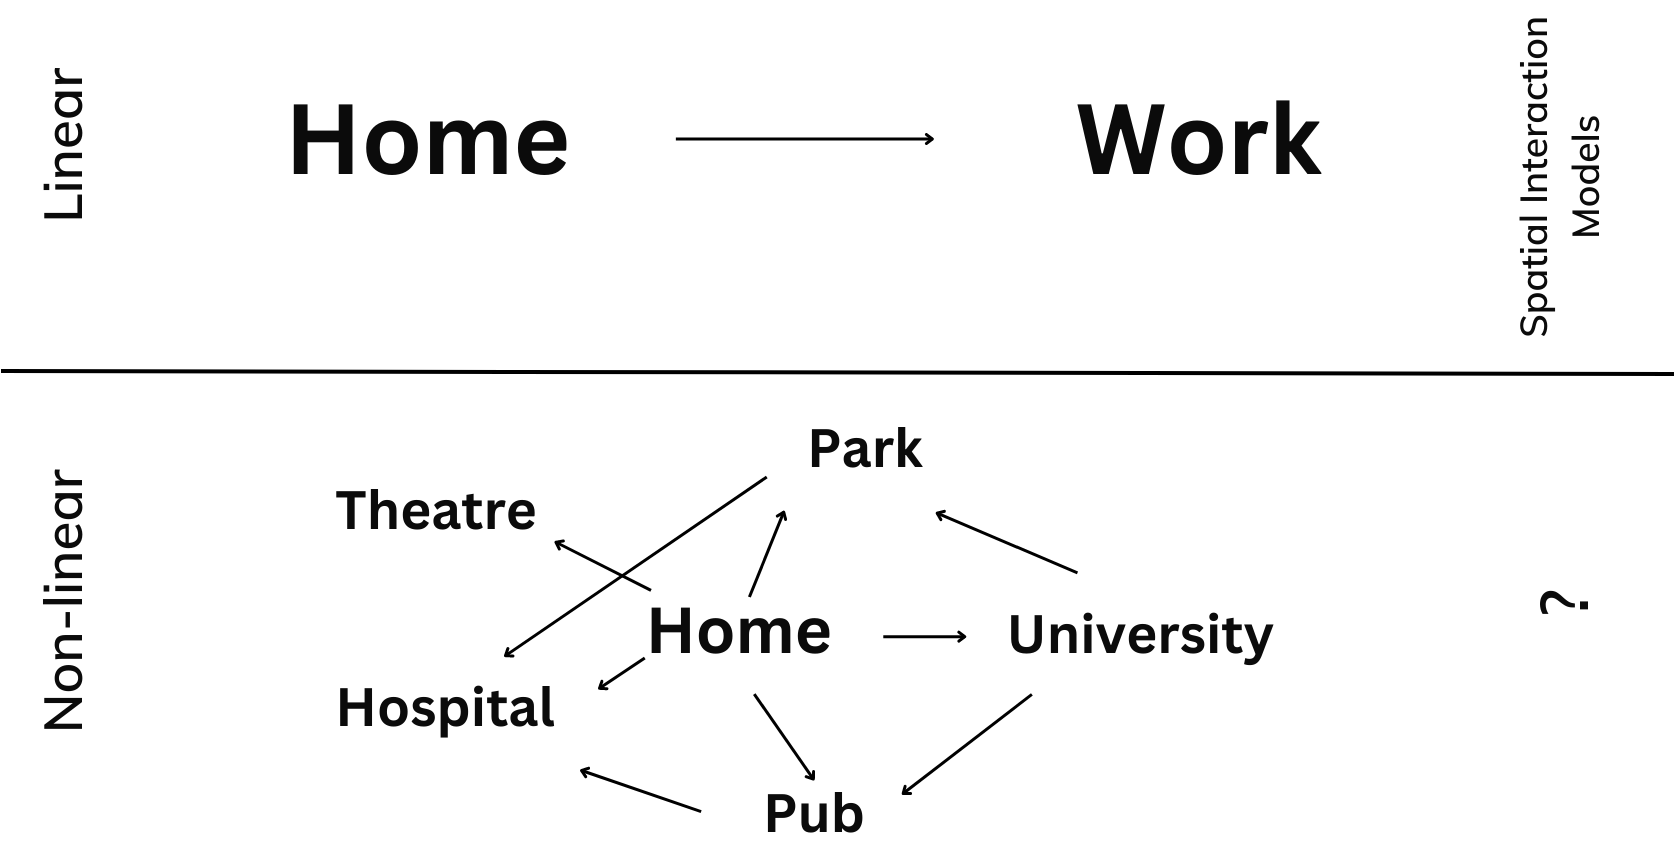
\includegraphics[width=12cm]{Images/context.png}
        \caption{Work x non-work flows}
        \label{fig: context}
    \end{figure}

   Using a spatial interaction model to predict movement patterns has proven to be a valuable tool for urban planning and understanding how cities change. However, the rise of big data in today's technology-driven age, with access to vast amounts of previously unseen information, has posed challenges for traditional models. Therefore, new models such as the Deep Gravity Model, in which the Gravity Model is combined with neural network architecture, show great promise in efficiently estimating mobility flows. As a result, innovative approaches that involve artificial intelligence and machine learning are being explored to update transportation modelling methods. These modern methods hold great potential for revolutionising the way we model and plan for transportation in cities.

In summary, urban mobility is a multifaceted challenge. Regular commuting forms a predictable pattern, but other types of travel involve diverse motivations and schedules. By embracing innovative techniques, we can unravel the complexities of various movements within cities. This adaptable approach to understanding mobility enhances our planning and accommodates the evolving dynamics of urban life and travel.
    
Hence, the main objective of this study is to assess the effectiveness of the deep gravity model in predicting mobility patterns for non-work-related flows. In this regard, evaluating the Deep Gravity model's performance against traditional Spatial Interaction Models assumes significant importance. 

This comparison between work-related and non-work-related flows offers a comprehensive understanding of the model's capabilities in estimating complex mobility patterns. Such an analysis is crucial in investigating the potential value that deep learning methodologies bring to non-work-related flow prediction and estimation.


    \section{Research Question}    

    How do Deep Gravity and Spatial Interaction Models differ in their predictive capabilities for estimating mobility flows, considering non-work-related and work-related trips?

   

    \section{Report Structure}

    \begin{itemize}
        \item \textbf{Chapter 2:} Literature Review - This chapter overviews key methodologies and limitations in estimating mobility flows. It delves into the structure of the spatial interaction model while introducing the application of deep learning to mobility flow analysis. Additionally, the chapter introduces the deep gravity model as another method for flow estimation. 
        \item \textbf{Chapter 3:} Methodology - This chapter explains the architectural foundations of both models. It also delves into the dataset employed in this study and how it was structured for utilisation in both models. The chapter concludes by outlining the evaluation metrics that will be used to assess the performance of these models.
        \item \textbf{Chapter 4:} Results and Discussion - First, the evaluation of the models takes centre stage. The chapter showcases visualisations of the generated flows and presents the principal findings alongside their associated limitations.
        \item \textbf{Chapter 5:} Conclusion - The concluding chapter summarises the significance of the analysis undertaken. It also underscores potential avenues for further investigation in the following studies.  
    \end{itemize}




% Some stuff about things.\cite{example-citation} Some more things. 

% Inline citation: \bibentry{example-citation}


\chapter{Literature Review}
\label{chapterlabel2}
    \section{Estimate mobility Flows} 

     Flow generation aims to synthesise real flow patterns between different geographical locations. It involves considering the specific attributes of these locations, such as population density, Points of Interest (POIs), land use characteristics, and the distances among them. This process is executed without direct access to real-world flow data, highlighting the dependence on generative models to represent mobility patterns accurately \citep{lucaSurveyDeepLearning2021}.
    
    Moreover, Mobility data captured through electronic devices provide invaluable insights into the movements of individuals over specific time intervals\citep{lucaSurveyDeepLearning2021}. These movements are recorded as spatiotemporal trajectories or aggregated mobility flows. Spatiotemporal trajectories and spatial aggregations, such as spatial-temporal points and tessellation, are crucial in this analysis as foundational elements for analysing and modelling mobility patterns\citep{lucaSurveyDeepLearning2021, siminiDeepGravityModel2021}.
    
    The implications of flow generation extend across various sectors, including urban planning, spatial economics, sustainable community design, and epidemiological modelling. The ability to generate accurate mobility flows is critical for addressing issues related to transportation planning, reducing socioeconomic inequalities, designing resilient communities, and understanding the spread of diseases within populations\citep{lucaSurveyDeepLearning2021}. Thus, the focus on flow generation and the generation of realistic mobility trajectories holds promise for enhancing various aspects of urban planning, spatial analysis, and public health.
      
    \section{Spatial Interaction models}

    A significant moment in the research of flow estimation was in 1946 when George K. Zipf introduced a conceptual framework for estimating mobility flows\citep{siminiDeepGravityModel2021, wilkinsonSpatialInteractionModels2023}. This model illustrated a parallel with Newton's universally accepted law of gravitation. This model, known as the gravity model, assumes that the amount of travellers moving between two specific locations is directly proportional to the population size of these locations. In parallel, this flow decreases in inverse proportion to their spatial separation\citep{wilsonFamilySpatialInteraction1971b}.
        
    While the gravity model has gained considerable attention due to its notable outcomes, some limitations exist. In particular, the gravity model needs help accurately capture some patterns inherent in real-world flows\citep{wilkinsonSpatialInteractionModels2023}. Furthermore, the generative process of flows, as predicted by the gravity model, does not consider the influence of other factors, such as Points of Interest (POIs), street networks, and other contextual variables\citep{lucaSurveyDeepLearning2021}.

    Besides that, spatial interaction models have some limitations in handling extensive datasets, such as loyalty card information, where basic calibration techniques can face constraints due to computational capabilities. \citep{wilkinsonSpatialInteractionModels2023}
    
    In parallel, some alternatives, such as the production-constrained model, have emerged to improve and extend the gravity model's efficacy. The Production-Constrained Model, conceived by \cite{wilsonFamilySpatialInteraction1971b}, introduces a key adjustment to traditional modelling techniques. Instead of relying on a single constant of proportionality, denoted as K, this model substitutes it with a set of constants commonly referred to as 'balancing factors.' This innovative approach allows more integration of additional knowledge as constraints within the modelling framework.

    The production-constrained or retail model considers critical input data, specifically the population distribution and corresponding purchasing power, to arrive at meaningful insights\citep{wilsonFamilySpatialInteraction1971b}. Related to transport, the production-attraction-constrained model serves as a valuable tool. It operates assuming that 'trip ends,' which denote the predetermined number of origins and destinations within each zone for a given type of trip, are available as input data. The primary aim of this model is to estimate the attractiveness factor based on this crucial information. To illustrate, constructing a model to analyse commuting patterns corresponds to the number of residents working in a region and the number of jobs\citep{wilsonFamilySpatialInteraction1971b}. This innovative approach provides a more comprehensive understanding of the dynamics involved in various scenarios and underscores the versatility of the production-constrained model in diverse analytical contexts.



    \section{Deep Learning for mobility flows}

    The application of neural network methodology in spatial interaction modelling marked a significant advancement in data science methodologies. A new approach from traditional models could provide more accurate predictions. \citep{wilkinsonSpatialInteractionModels2023}
        
    Comparative studies between neural network models and established frameworks revealed promising insights. These investigations indicated that neural networks could surpass the predictive accuracy of the Wilsonian model (Fischer \& Gopal, 1994; Black, 1995). However, it is crucial to note that these neural network models were frequently contrasted against unconstrained Ordinary Least Squares (OLS) calibrated models, raising queries about the true advantages of neural networks in spatial interaction modelling (Mozolin et al., 2000). \citep{wilkinsonSpatialInteractionModels2023}
        
    Incorporating neural networks presents specific challenges. The key requirement is the development of loss functions that are unambiguous, relevant, and clear. These functions play a pivotal role in estimating the total income of retail stores. The complexities of this implementation are highlighted in the iterative calibration phase, where the reliance on metrics such as average trip distance is emphasised. Thus, it is crucial to carefully consider and calibrate neural networks to ensure accurate revenue estimation in the grocery retail sector. \citep{wilkinsonSpatialInteractionModels2023}
        
    The early applications of neural networks in spatial interaction modelling demonstrated their potential to enhance predictive accuracy in commodity flows, trade, and migration domains. However, a comprehensive understanding of their advantages over traditional models requires more nuanced comparative assessments\citep{wilkinsonSpatialInteractionModels2023}.

    Deep Learning models offer the advantage of a high perfomance in capturing complex mobility patterns, a valuable method for flow generation. However, it is important to note their effectiveness on the data they are trained on, raising questions about their applicability across different geographical contexts. \citep{wilkinsonSpatialInteractionModels2023}

    \cite{lucaSurveyDeepLearning2021} study aims to investigate the use of deep learning techniques in mobility-related tasks. The research focuses on estimating mobility flows, particularly on generating realistic trajectories that replicate actual movement patterns. The study aims to enhance our understanding of complex mobility networks and their applications in various domains by utilising deep learning.

    Besides that, an inherent characteristic of Deep Learning models is their opacity, often called "black boxes". As stated by \cite{lucaSurveyDeepLearning2021}, This opacity can make interpreting the underlying logic behind generating trajectories or predicting locations and flows challenging. Nevertheless, interpretability is essential to comprehend mobility patterns and uncover potential biases in the model's decision-making process.
        
    According to \cite{lucaSurveyDeepLearning2021}, while Deep Learning models offer promise, they also introduce privacy concerns during the training and prediction phases. For instance, a critical issue in trajectory generation lies in assessing the risk of re-identifying real individuals from synthetic trajectory data. This concern becomes even more pronounced when data availability for model training is limited.
        
    The evaluation of flow generators typically relies on commuting data obtained from official statistical institutes' censuses. The assessment of flow generation commonly revolves around calculating the Common Part Of Commuters (CPC) between real and generated flows. Additionally, widely used metrics like Mean Absolute Error (MAE), Root Mean Square Error (RMSE), and Mean Absolute Percentage Error (MAPE) are also employed for this purpose.
        
    To summarise, integrating Deep Learning into generative tasks related to mobility patterns is a relatively recent development poised to gain prominence in the near future. While these models hold the potential to unravel complex mobility dynamics, their reliance on training data, lack of transparency, privacy considerations, and evaluation metrics emphasise the multifaceted nature of their application in this domain.   

    \begin{figure}[H]
        \centering
        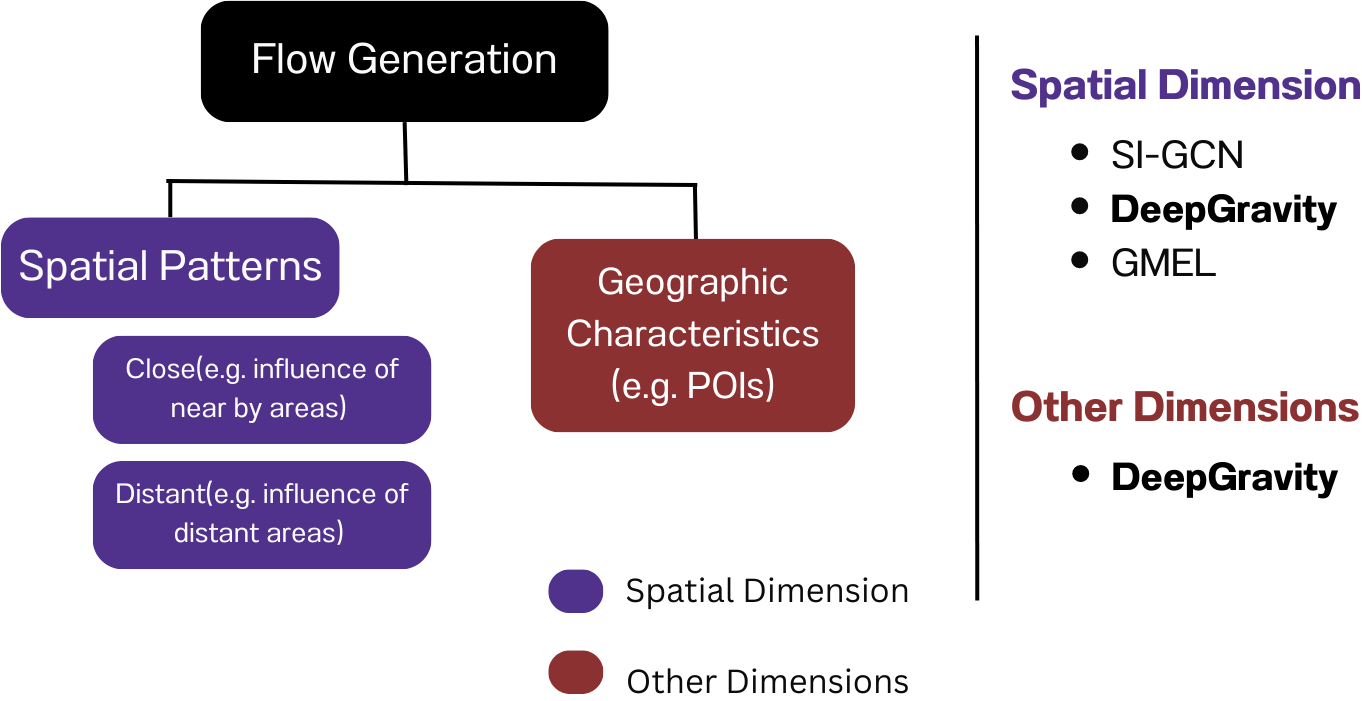
\includegraphics[width=12cm]{Images/deepgravity_fig.png}
        \caption{Deep Learning for Mobility Flows. Adapted from: \cite{lucaSurveyDeepLearning2021}}
        \label{fig: DG evaluation}
    \end{figure}

        
    \section{Deep Gravity Model}

    Deep learning methodologies have marked a significant landmark in mobility studies, particularly in analysing and predicting mobility flows. Some studies have presented the potential of deep learning techniques to encapsulate complex relationships embedded within mobility data while also drawing attention to the challenges inherent in the inherent opacity of these models, such as privacy concerns and the salient role of geographic features in enhancing the fidelity of flow predictions.

    Luca et al.'s study underscores the unique capacity of deep learning models to navigate intricate and non-linear associations within the data. This feature enables the seamless assimilation of supplementary data about specific locations, such as population density and Points of Interest (POIs). This feat eludes conventional spatial interaction models. This novel approach drives the understanding of mobility patterns beyond the linear models, providing a more holistic comprehension\citep{lucaSurveyDeepLearning2021}.

    \cite{lucaSurveyDeepLearning2021}'s work lies in the innovative concept of the Common Part of Commuters (CPC), an instrumental metric that assesses flow generator performance. This metric involves a comparative analysis of the model-generated flows against real-world data, thereby quantifying the accuracy of predictions. In addition to CPC, the study underscores the significance of employing a diverse array of evaluation metrics, including Mean Absolute Error (MAE), Root Mean Squared Error (RMSE), and Mean Absolute Percentage Error (MAPE), to offer a comprehensive understanding of model efficacy (Luca et al., 2021). 

    Beyond the technical aspects, the research presents the challenges tied to the inherent opacity of deep learning models, spotlighting the critical need to address privacy concerns, especially in scenarios involving trajectory generation where limited data availability poses a formidable obstacle (Luca et al., 2021).

    Simini et al.'s work, adds a new dimension to the discourse by delving into flow prediction and generation. A key aspect of their approach is the strategic application of geographic features extracted from OpenStreetMap to improve the accuracy of mobility flow predictions. This strategic incorporation of geographical attributes forms the bedrock upon which the Deep Gravity model, a deep neural network, is trained.
 
    The acknowledgement of the opacity challenge intrinsic to deep learning models is worth highlighting, which they address by supporting the input of explainable AI techniques to enhance the interpretability and transparency of the model's decision-making process (Simini et al., 2021).

    Regarding model performance, Simini et al.'s research shed light on the superior efficacy of the Deep Gravity model vis-à-vis conventional shallow neural networks and established gravity models. This contrast in performance underscores the intrinsic potency of deep learning in uncovering nuanced relationships within geographical attributes, ultimately yielding more precise flow predictions (Simini et al., 2021). .

    The study also highlights the pivotal role of the intricate interplay of diverse geographic features, particularly in densely populated regions. This intricate dance of geographic attributes significantly enhances the model's predictive capabilities, especially in scenarios where traditional models fall short (Simini et al., 2021).

    In summary, the combined endeavours of Luca et al. (2021) and Simini et al. (2021) offer an insightful glimpse into the potential of deep learning models to decode and simulate the complex tapestry of mobility flows. These studies collectively illuminate the capacity of these models to untangle intricate relationships embedded within mobility data and underscore the significance of embedding geographic features to elevate the precision of flow predictions.

    While these studies grapple with the challenges of model opacity and privacy concerns, they collectively herald the transformative potential of deep learning in enhancing our understanding of mobility patterns. By extrapolating from these findings, the Deep Gravity model emerges as a promising contender for replication across a diverse spectrum of contexts, effectively transcending the constraints of census data that formed the foundation of the original studies. 

    This extension holds the promise of extracting invaluable insights from high-accuracy datasets, as exemplified in the bustling urban milieu of London, potentially revolutionising the landscape of urban planning and decision-making.



    \section{Conclusion}

    In this literature review, we have explored the importance of estimating mobility flows and the relevance of spatial interaction models in this context, focusing on recent developments in deep learning models. Flow estimation, crucial for understanding urban mobility, involves synthesising patterns of movement between different geographical locations, considering factors such as population density, Points of Interest (POIs), land use, and distances. These flow patterns play a pivotal role in various domains, including urban planning, spatial economics, community design, and epidemiological modelling, addressing challenges related to transportation planning, socioeconomic disparities, community resilience, and disease spread.

    Spatial interaction models offer valuable insights into flow estimation but have limitations in capturing complex real-world patterns and considering contextual factors like POIs and street networks. On the other hand, Deep learning models have brought significant advancements in mobility flow estimation, surpassing traditional models' predictive accuracy. These models excel in capturing complex relationships within mobility data, albeit with concerns about their opacity and privacy implications.

    The Deep Gravity model, combining geographic features from OpenStreetMap with deep neural networks, demonstrates superior performance in flow prediction compared to conventional models, further emphasizing the potential of deep learning in unravelling nuanced relationships within geographical attributes. The studies collectively suggest that these models can improve our understanding of mobility patterns, especially when applied to high-accuracy datasets in urban planning and decision-making contexts.
\chapter{Methodology}
\label{chapterlabel3}

This study analyses the performance exhibited by the Deep Gravity and Production-constrained models concerning work-related and non-work-related flows within London. As a result, this work establishes a comprehensive comparison between the outcomes generated by these models and the observed flow patterns present in the context of London. This comparative investigation provides a more robust understanding of the efficacy and applicability of the Deep Gravity and Production-constrained models.



% STUDY AREA

    \section{Study Area}

This study focuses on the entire region of London,  its inner and outer areas. London has diverse cultures, nationalities, incomes, transportation options, public services, and amenities. To truly understand how people travel across the city, looking at the entire region is essential. This approach intends to understand the commuting patterns, considering all the factors contributing to how people move around in this diverse and dynamic urban environment.


%%% DATA

    \section{Data}

This study relies on three primary datasets: Locomizer, Point of Interest, and Census 2021. Locomizer serves as the central component of the analysis, with the aggregated origin and destination flow for London within hexagons as geographic area units. The hexagon ID serves as the primary index, and to ensure coherence, the remaining datasets are incorporated into this index via an area-weighted spatial join.

    \begin{figure}[H]
        \centering
        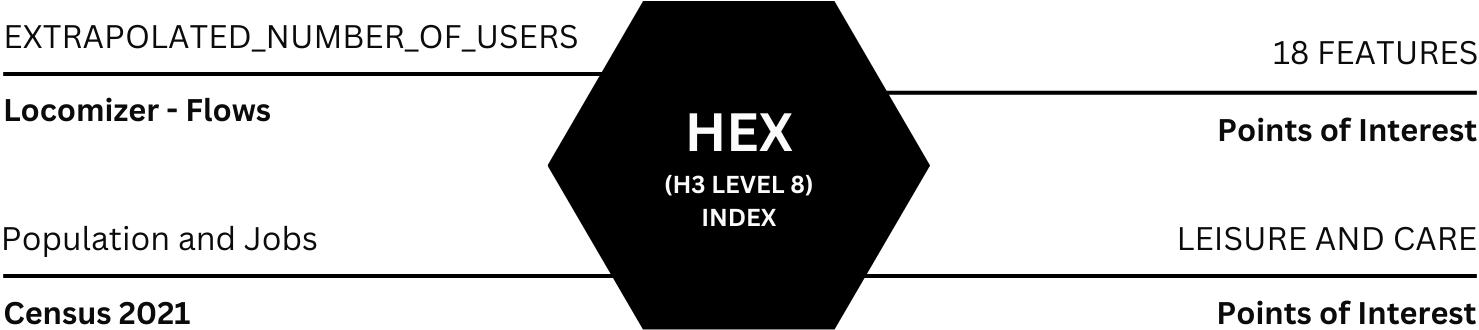
\includegraphics[width=12cm]{Images/framework.png}
        \caption{Methodology framework}
        \label{fig: framework}
    \end{figure}


%%% Mobility Data
     \subsection{Mobility data} 

The Locomizer is a  human mobility dataset derived from mobile phone devices, ensuring that the participants have explicitly consented to utilise their data. This dataset contains a variety of key metrics. It captures observed and extrapolated counts of users who have spent time within a specified geographic area over a specific timeframe. Moreover, it includes the number of signals, effectively representing observations, at each location.

These metrics are organised based on different movement categories, distinguishing between pedestrian and non-pedestrian activities. Additionally, the dataset categorises users based on visitation modalities,  differentiating "workers" from the overall population. Identifying the "common daytime location (CDL)" or the workplace for these worker users is accomplished by analysing device-level data and areas with the highest dwell time during typical working hours. This specific analysis aids in understanding and inferring the work-related locations of these users. To decrease granularity, worker users are aggregated, and the resulting data is presented at the point level, utilising a 69-meter radius around each point of interest (POI).

The dataset applied in this study contains aggregated data at level 9(Figure \ref{fig: grid 7}, with each dataset file including more than 4 million rows. The careful cleaning of this dataset emerged as an essential requirement to ensure the integrity of subsequent analyses. Hexagons play a key role in understanding spatial relationships, particularly mobility flows. Despite the computational limitation of running the spatial interaction model to deal with a high amount of data,  it required a transition from hexagonal level 9 to level 7. This transformation was facilitated through the H3 package\citep{uberTablesCellStatistics2023} in Python. At level 9, a hexagon has a relatively small area, approximately 0.10 square kilometres. In contrast, at level 7, a hexagon covers a significantly larger area, approximately 5.16 square kilometres.

    \begin{figure}[H]
        \centering
        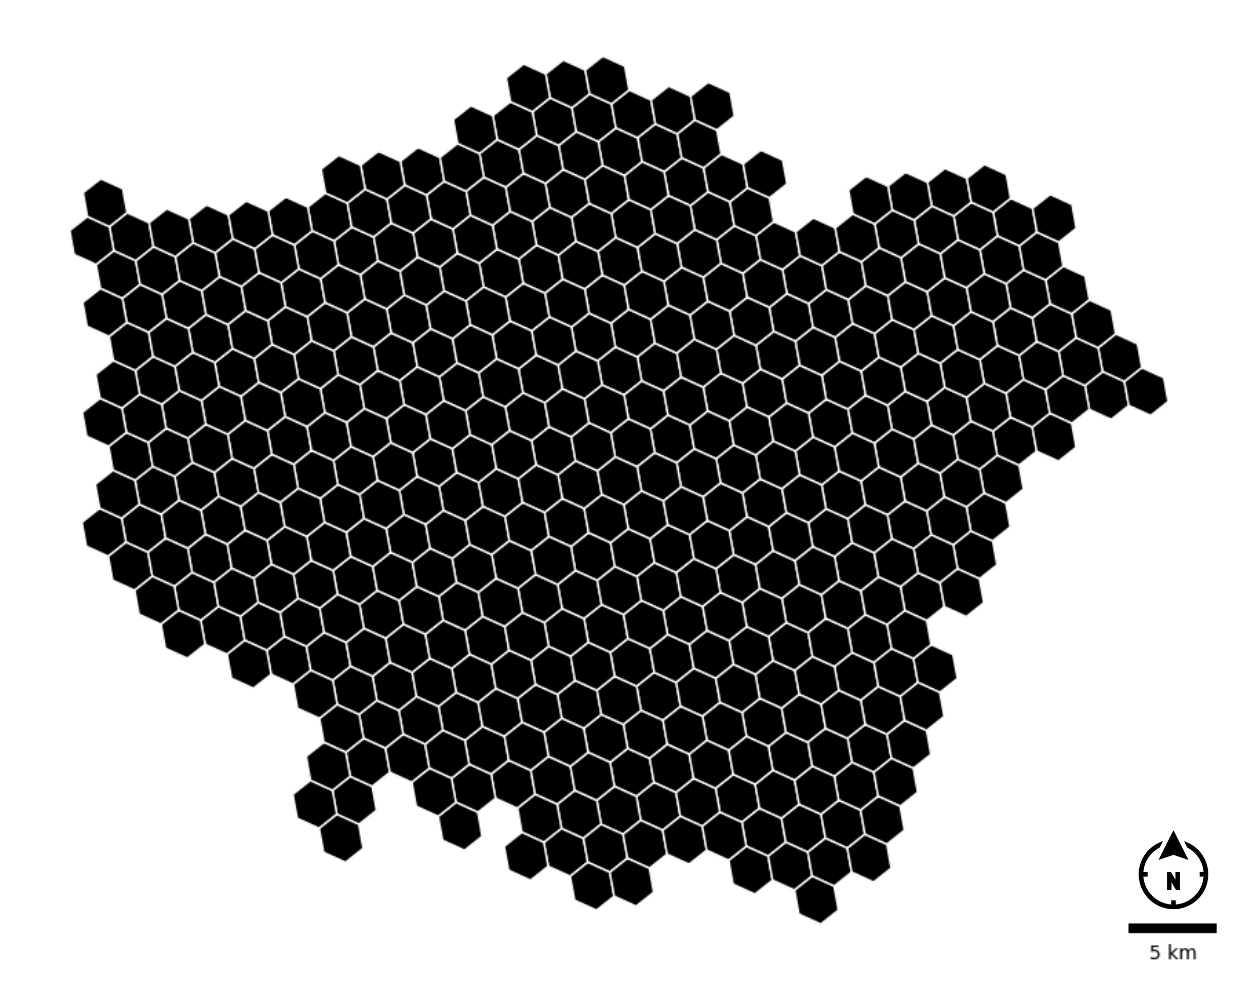
\includegraphics[width=10cm]{Images/Hexagons_level7.png}
        \caption{London in Hexagons at level 7}
        \label{fig: grid 7}
    \end{figure}  
    
The dataset contains two fundamental segments: the origins, while the other relates to destinations. Both datasets are characterised by columns ORIGIN and DESTINATION. However, only the top 100 destinations were retained within the' Origin' segment. On the other hand, only the top 100 origins were incorporated in the' Destination' segment. This approach provides a more comprehensive overview of the system's dynamics. Flows lacking a defined origin or destination, denoted by '0' entries, were excluded. Moreover, it eliminated duplicated flow instances from the final dataset.

The 'extrapolated number of users' concept is introduced to estimate user presence within a specific geographic region over a designated time frame. Diverse movement modalities are available in the dataset, with the entirety ('all') and the workforce ('workers'). The 'transient' aspect, defined as the difference between the overall movement and the workforce, is established for non-work flows. The dataset explores variations in movement modes, such as walking/non-walking. However, this study considers the 'All' categorization to investigate the general mobility patterns.

It was chosen to focus only on data from a single day despite the availability of extensive datasets. Wednesday was chosen as the focus day to represent a regular workday without exceptional events, such as strikes. Additionally, Sunday was considered suitable for examining non-work-related movements, providing insights into mobility unaffected by work duties.

The Table \ref{table: Locomizer features} below summarizes the main aspects of the dataset. It provides insights into the utilized hexagonal grid, the identifiers for origin and destination points, the mode of movement, the temporal scope of analysis, and the specific days selected for work-related and non-work-related flows.





\begin{table}[H]
\centering
\begin{tabular}{ll}
\hline
\textbf{Features}   & \textbf{Description}        \\ \hline
\textbf{Grid}               & Uber H3 hexagons at Level 8 \\
\textbf{Origin\_Code}        & Origin HEX ID               \\
\textbf{Destination\_Code}   & Destination HEX ID          \\
\textbf{Visitation Modality} & All                         \\
\textbf{Movement Modality}   & All/ Workers/ Transients¹   \\
\textbf{Daytime}             & 25 (00.00-23.59)            \\ 
\textbf{Work Flow Date}      & 08/03/2023 (Wednesday)      \\ 
\textbf{Non-work Flow Date}  & 12/03/2023 (Sunday)         \\ \bottomrule
\end{tabular}
    \caption{Features classification - Locomizer Dataset}
    \label{table: Locomizer features}
\end{table}

Hexagons at level 7 in London have 415 hexagons, resulting in 172,225 possible origin and destination flow combinations. Consequently, the dataset concerning work and workflows displays a distinct distribution, as shown in Figure \ref{fig: Data Values Overview}. This distinction arises because workflows constitute only a fraction of the overall flow. As a result, this dataset showcases both a reduced maximum value and a lower mean value. This value difference leads to a more balanced workflow data distribution, as the accompanying graph shows. Furthermore, the distance from the mean (standard deviation) is notably smaller. Therefore, the values shown in the graphs are presented in logarithmic scale to accommodate the dataset's extensive size and prevent value distortion.


    \begin{figure}[H]
        \centering
        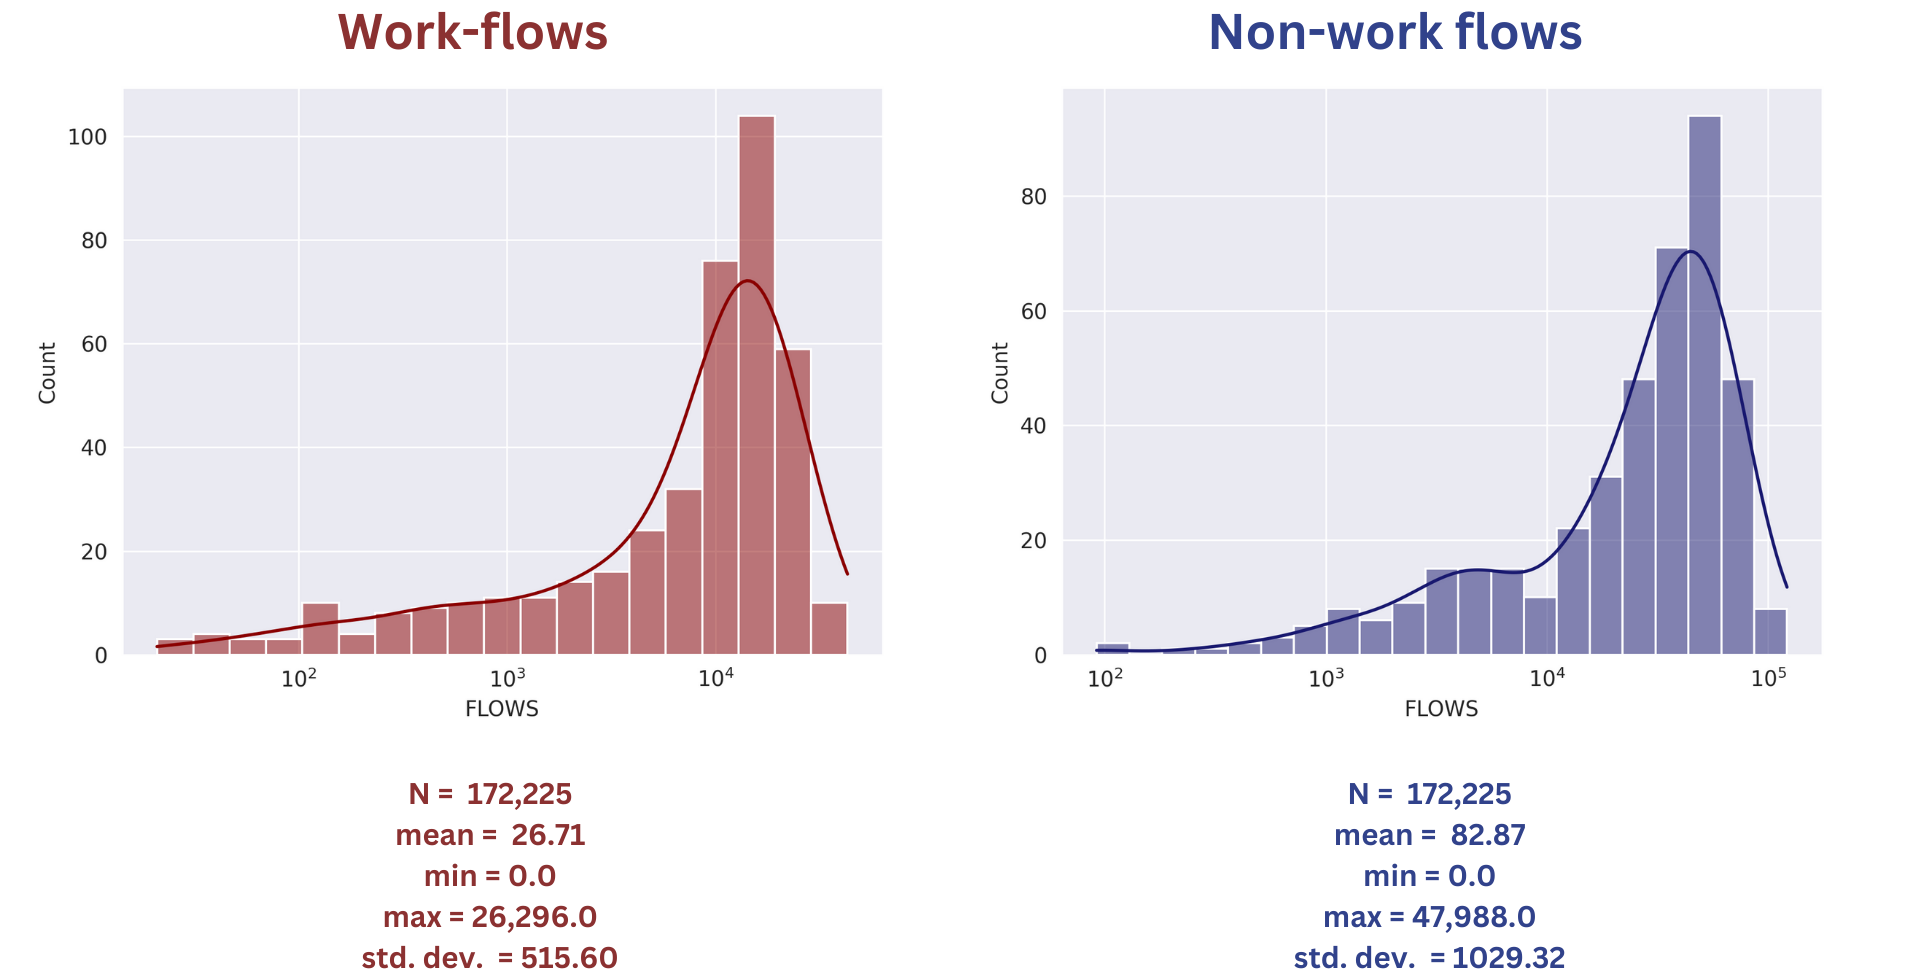
\includegraphics[width=15cm]{Images/Data_values_overview.png}
        \caption{Data Values}
        \label{fig: Data Values Overview}
    \end{figure}

 %%% POINTS OF INTEREST
 
        \subsection{Points of Interest(POI)} 

        The Points of Interest is a dataset categorising various establishments and services across Great Britain, both public and private. The classification system is structured across three levels, each contributing to a comprehensive categorisation of various entities\citep{osPointsInterestClassification2022}.
        
        At the initial level, nine broad Groups serve as the foundation for classification, see Table \ref{table: POIs_groups} . These Groups contain diverse areas such as accommodation, eating and drinking establishments, commercial services, attractions, sports and entertainment facilities, education and health institutions, public infrastructure sites, manufacturing and production facilities, and retail and transport services.

        \begin{table}[H]
\centering
\begin{tabular}{@{}lll@{}}
\toprule
\textbf{COD} & \textbf{Categories} & \textbf{Examples} \\ \midrule
AED & Accommodation, Eating and Drinking & Hotels, Cafes, Pubs \\
CS & Commercial services & Construction, marketing services \\
AT & Attractions & Art Galleries, Zoos, museums  \\
SE & Sport and Entertainment & Sports Complex, Cinemas \\
EH & Education and Health & Health centres, Primary Schools \\
PI & Public infrastructure & Police stations, Wi-Fi hotspots \\
MP & Manufacturing and production &  Conservatories, Farming \\
RT &  Retail & Bakeries, Department stores \\
TR & Transport & Bus stops, Tube stations \\ \bottomrule
\end{tabular}
    \caption{POI categories}
    \label{table: POIs_groups}
\end{table}
        
        Moving to the next level, Level 2, this classification system becomes more refined, consisting of 52 distinct Categories. These Categories further study the entities, providing a more detailed perspective within each Group. Within these categories, specific subcategories define each entity's characteristics. Finally, Level 3 is the most specific classification level, featuring 600 individual Classes. This categorisation ensures a high level of granularity, allowing for precise differentiation and more understanding of the entities within the dataset.

        A hierarchical structure of three distinct levels is evident within this framework\citep{osPointsInterestProduct2022}, as shown in Figure \ref{fig: POI levels}. To provide a concrete example, let us examine the hierarchy within the context of transportation. At the highest level, we have the "Transport" category, a broad umbrella term. Moving down the hierarchy, we encounter the more specific "Category" known as "Bus Transport," which limits the focus to a subset of bus-related transportation. Finally, we reach the most granular level, "Class," exemplified by "Bus Stops". This hierarchical arrangement offers a versatile spectrum of possibilities and classification options, allowing for a comprehensive and structured approach to organising information within the given system.

        \begin{figure}[H]
            \centering
            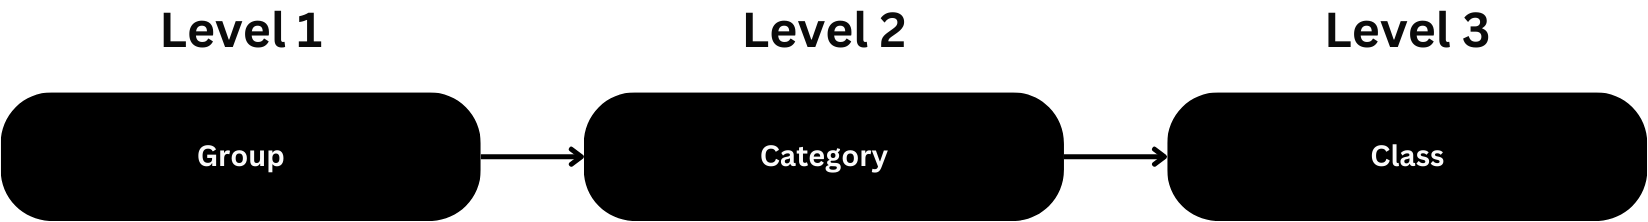
\includegraphics[width=12cm]{Images/POI_levels.png}
            \caption{POI levels}
            \label{fig: POI levels}
        \end{figure}


        Due to its increased complexity and adaptability to diverse geographic characteristics, the deep gravity model requires a comprehensive approach when applied to the POI dataset. This model requires a total set of 18 unique geographic features, each contributing specific information about each geographic unit, which, in this context, are represented by hexagons. 
        We derived a classification based on the one in \cite{siminiDeepGravityModel2021} and the one given by the Ordnance Survey, see Table \ref{table: class_POIs}. 

        Therefore, the approach involves considering all available data points for extraction. The categories were restructured because the POI dataset initially included only nine distinct groups, while the Deep Gravity Model required 18 features as input. This restructuring aimed to optimise compatibility with the Deep Gravity Model and provide an equitable information distribution across the new features.


\begin{table}[H]
\centering
\begin{tabular}{@{}ll@{}}
\toprule
\textbf{Item} & \textbf{Category}                             \\ \midrule
1             & Bus Transport                                 \\
2             & Public Transport, Stations and Infrastructure \\
3             & Water                                         \\
4             & Air                                           \\
5             & Education                                     \\
6             & Health                                        \\
7             & Accomodation                                  \\
8             & Restaurants                                   \\
9             & Fast Food                                     \\
10            & Pubs, Bars and Inns                           \\
11            & Cafes, Snack Bars and Tea Rooms               \\
12            & Retail                                        \\
13            & Commercial Services                           \\
14            & Sport and Entertainment                       \\
15            & Attractions                                    \\
16            & Infrastructure and Facilities                 \\
17            & Central and Local Government                  \\
18            & Organisations                                 \\ \bottomrule
\end{tabular}
    \caption{Features classification based on POI dataset}
    \label{table: class_POIs}
\end{table}

        The "Transport" category was disaggregated into four distinct features, each designed to encapsulate the richness of information originally associated with the broader transport aspect. These features effectively retained the essence of the original category names. Moreover, the "Education and Health" group has a similar transformation, grouping many correlated points of interest. Recognising that users often have varying motivations for visiting such locations, this group was split into two separate features: one dedicated to Education and the other to Health.
        
        "Accommodation, Eating, and Drinking" showed many non-work-related opportunities, rendering it one of the most densely populated categories. As a result, this group was divided into four features, reflecting the underlying categories. On the other hand, "Retail," "Commercial Services," and "Attractions" were considered to retain their original classification without further splitting, maintaining a simplified representation. Moreover, the "Public Infrastructure" category garnered significant attention in the regression analysis(Tables \ref{tab:ols-results} and \ref{tab:ols-results-new-bold-color}), categorising it into three distinct features. 
        
        The detailed structure of the feature classification is available in the appendices \ref{appendices1}. It is important to highlight that this new classification strategy does not consider the "level class" despite the limitations in feature count and the analytical complexity. 
    
        Within the Spatial Interaction Model (SIM) framework, the Point of Interest (POI) dataset aggregates the cumulative counts of points relevant to work-related and non-work-related amenities. This categorisation was the foundation for a statistical analysis to unveil the relationships between specific POI groups and Mobility Data Flows. Two separate regression analyses were conducted—one tailored to work-related flows and another to non-work flows.
        
        


 %%% CENSUS DATA
        \subsection{Census data} 
    
    The census data plays a crucial role in both models. In the spatial interaction model, the population is one of the independent variables used to calculate predicted flows alongside factors like distance and attractiveness. Meanwhile, the Deep Gravity Model population data contributes to the location feature vector, which offers a spatial representation for each hexagon. This feature vector includes information from the Points of Interest (POI) dataset and the population size of hexagons obtained from the 2021 census.

    Data consistency is vital, given that the mobility data collected is from 2023, while the Points of Interest data is from 2022. Therefore, including the 2021 census data on London's population becomes crucial for maintaining coherence in the final data analysis. Thus, to prepare the data for use in the models, it was necessary to aggregate it under a common index—specifically, the Mobility data index in Hexagons at level 7. This aggregation step ensures the data is structured consistently for both models' analyses.

    Moreover, population data include an integral part of the 'Population and household estimates for England and Wales: Census 2021'. The Census employs a definition of a usual resident, encompassing individuals who were in the UK on Census Day (21 March 2021) and intended to stay for at least 12 months. Meanwhile, a household is defined as a single person living alone or a collective group.

    \section{Research scope}

%%%%%% DEEP GRAVITY    
        \subsection{Deep gravity Model}


The Deep Gravity model uses various input features to compute the probability $p_{i,j}$ a trip originating at a given location (e.g., $l_i$), to end at any of the $n$ other locations in the region of interest (e.g., $l_j$). The model produces an $n$-dimensional vector of probabilities $p_{i,j}$ for each $j = 1, ..., n$, and this computation is carried out in three steps.
In the first step, input vectors $x(l_i, l_j)$ are created by combining three input features:

\begin{itemize}
        \item $x_i$, representing the feature vector of the origin location $l_i$
        \item $x_j$, representing the feature vector of the destination location $l_j$
\end{itemize}
The geographic distance $r_{i,j}$ between the origin and destination
For each origin location ($l_i$), $n$ input vectors $x(l_i, l_j)$ with $j = 1, ..., n$ are generated, each corresponding to a possible destination within the region of interest.

Next, these input vectors $x(l_i, l_j)$ are fed in parallel into the same feed-forward neural network, consisting of 15 hidden layers. The output of the final layer is a scalar $s(l_i, l_j) \in [-\infty, +\infty]$, referred to as the score, which indicates the likelihood of observing a trip from $l_i$ to $l_j$ according to the model. The probability (i.e., the model's output) is multiplied by the origin's total outflow to determine the generated flow between two locations.

The location feature vector $x_i$ provides a spatial representation of an area and includes features describing properties of the location $l_i$. Its dimension, $d$, corresponds to the total number of considered features.

Additionally, Deep Gravity considers the geographic distance, $r_{i,j}$, between two locations, $l_i$ and $l_j$, measured along the earth's surface between the centroids of the two polygons representing the locations. Each flow in Deep Gravity is described by 39 features, comprising 18 geographic features of the origin and 18 of the destination, along with the distance between the origin and destination and their populations.

    \begin{figure}[H]
        \centering
        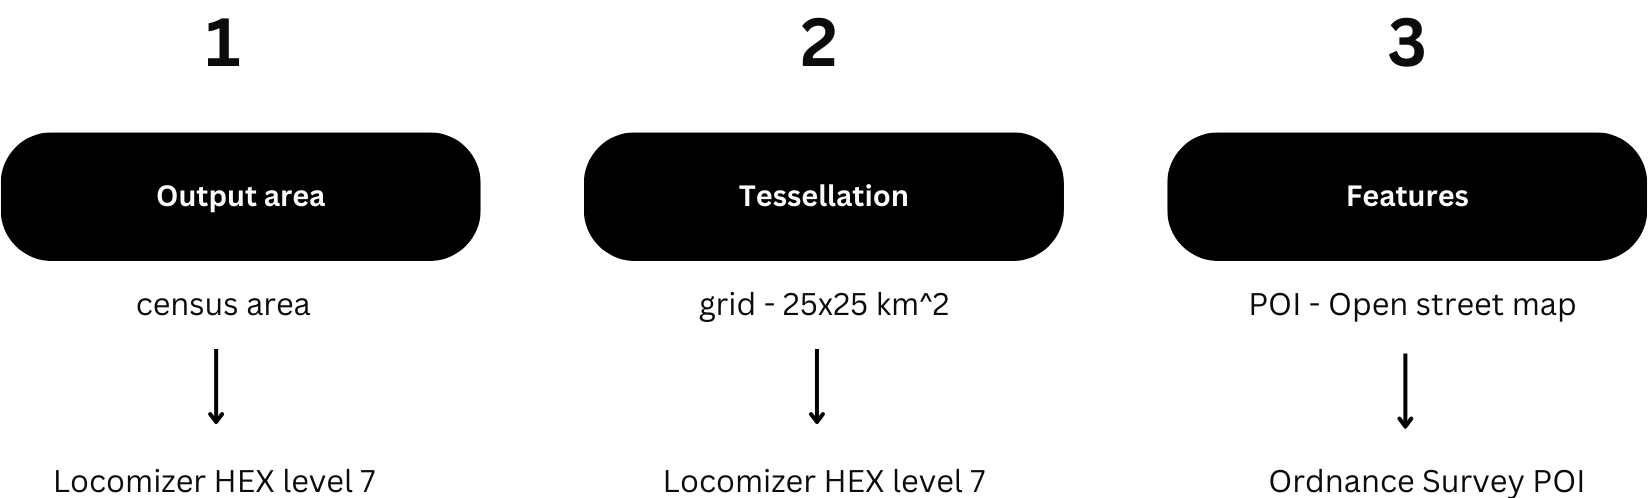
\includegraphics[width=14cm]{Images/DG_Input.png}
        \caption{Deep Gravity Model inputs}
        \label{fig: DG_input}
    \end{figure}

Moreover, deep gravity is a model developed using Pytorch. This Python library conducts real-time execution of dynamic tensor computations, incorporating automatic differentiation and GPU acceleration while maintaining performance levels on par with the fastest contemporary deep learning libraries\citep{paszkePyTorchImperativeStyle2019}.  
    
%%%%%%%%%SPATIAL INTERACTION MODEL

\subsection{Spatial Interaction Model}

The selected spatial interaction model for assessing commuting flows for work and non-work purposes is the production-constrained model, commonly called the retail model. This model offers the advantage of constraining origin information, employing categorical variables, the distance and incorporating data on destination attractiveness. It enables us to gain insights into the dynamics of commute flows from various origins to potential destinations. Our study determined destination attractiveness by considering the total counts of points of interest associated with each flow type, as outlined in the Dataset section.


The availability of the Mobility dataset plays a crucial role, enabling the collection of work and non-work flows between origin and destination hexagons. Consequently, the equation of this model can be expressed as follows:

\begin{equation} \label{eq:1} \tag{1}
T_{ij} = A_i O_i D_j^\gamma d_{ij}^{-\beta}
\end{equation}
where
\begin{equation} \label{eq:3} \tag{2}
A_i = \frac{1}{\sum_j D_j^\gamma d_{ij}^{-\beta}}
\end{equation}

\begin{itemize}
    \item $A_i$ stands for a vector of size $n$ containing the Hexagon origin balancing factors, essential for maintaining the total out-flows in the predicted flows.
    \item $O_i$  represents a vector of size $n$ that indicates the total number of flows originating from the origin $i$ ( Hexagon Origin ID).
    \item $f(d_{ij})=d_{ij}^{-\beta}$  is a function of cost or distance, referred to as the distance-decay function.
\end{itemize}

The model is calibrated using a Poisson Regression function

\begin{equation} \label{eq:4} \tag{4}
\lambda_{ij} = \exp (\alpha_i + \gamma \ln D_j - \beta \ln d_{ij})
\end{equation}
where $\alpha_i$

\begin{figure}[H]
        \centering
        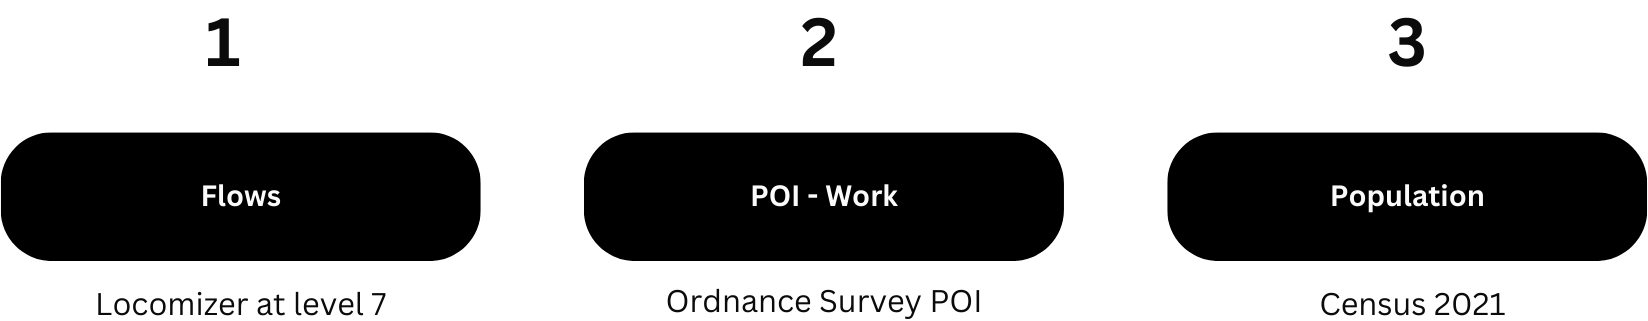
\includegraphics[width=14cm]{Images/SIM_fig.png}
        \caption{Spatial Interaction Model Inputs}
        \label{fig: SIM_input}
    \end{figure}


\subsection{Validation}

The main objective of this study is to use the Root Mean Squared Error (RMSE) to validate models designed for both work and non-work flows. Alongside RMSE, other frequently employed metrics include the Mean Average Error (MAE) and the Mean Average Percentage Error (MAPE). Several error metrics, such as MAE, Mean Squared Error (MSE), RMSE, and MAPE, are frequently employed within this context. These metrics operate within the $[0, \infty ]$ range, where in lower values indicate superior performance. Moreover, The evaluation of flow generation is also carried out by measuring the Common Part of Commuters (CPC) between real and generated flows\citep{lucaSurveyDeepLearning2021}.

As \cite{lucaSurveyDeepLearning2021} stated, MAE considers the absolute value of errors, neglecting the direction of overestimation or underestimation. On the other hand, MSE emphasizes larger errors more significantly than MAE and is also sensitive to outliers. RMSE, the focus of this study, places a greater emphasis on errors than MAE, penalizing models that produce substantial errors. This particular metric is expressed in the same units as the predicted values due to the squared nature of the calculation.

Therefore, this study's pursuit of employing RMSE to validate models dealing with work and non-work flows aligns with established evaluation practices. 

\subsection{Ethical Consideration}

The Locomizer dataset encompasses mobile device-derived information aggregated at hexagons levels, with data updates occurring hourly. The provider of this dataset, LOCOMIZER Ltd, has affirmed its adherence to the General Data Protection Regulation (GDPR) of 2018. This data repository comprises mobility data sourced from mobile devices, procured exclusively with explicit user consent and meticulous observance of local privacy regulations, including but not limited to GDPR.

The dataset adopts a spatial aggregation approach utilizing hexagonal cells, specifically at H3, level 9, and encompasses the geographical expanse of London. Each hexagonal cell corresponds to an approximate area of 0.1 km². The data's temporal granularity follows an hourly structure, which is subsequently summarized daily within the scope of a designated month. Consequently, the intrinsic design of the dataset precludes the identification of individualized locations.

In this context, the Locomizer dataset was obtained by Foster and Partners, the project partner of this dissertation project. This collaborative initiative has established prior authorization for data usage as stipulated within the agreement between the two parties. As a result, the ethical implications surrounding this study were considered low risk, culminating in the project's approval by the Committee for the Centre for Advanced Spatial Analysis (CASA) at University College London (UCL).
\chapter{Results and Discussion}
\label{chapterlabel4}
    \section{Parameters}
        \subsection{Flows}

        As evident from the observed movement patterns from the Mobility Dataset in Figure \ref{fig: observedflows_overview} , work-related and non-work-related flows exhibit a concentration of commuting trajectories within central London. Moreover, substantial flows are concentrated in the northeastern and southwestern regions of the city. The most notable difference between these two categories of flows lies in the concentration level: Work-related flows demonstrate a heightened level of convergence, whereas non-work-related flows display a distribution that extends spatially across a broader area.

    \begin{figure}[H]
        \centering
        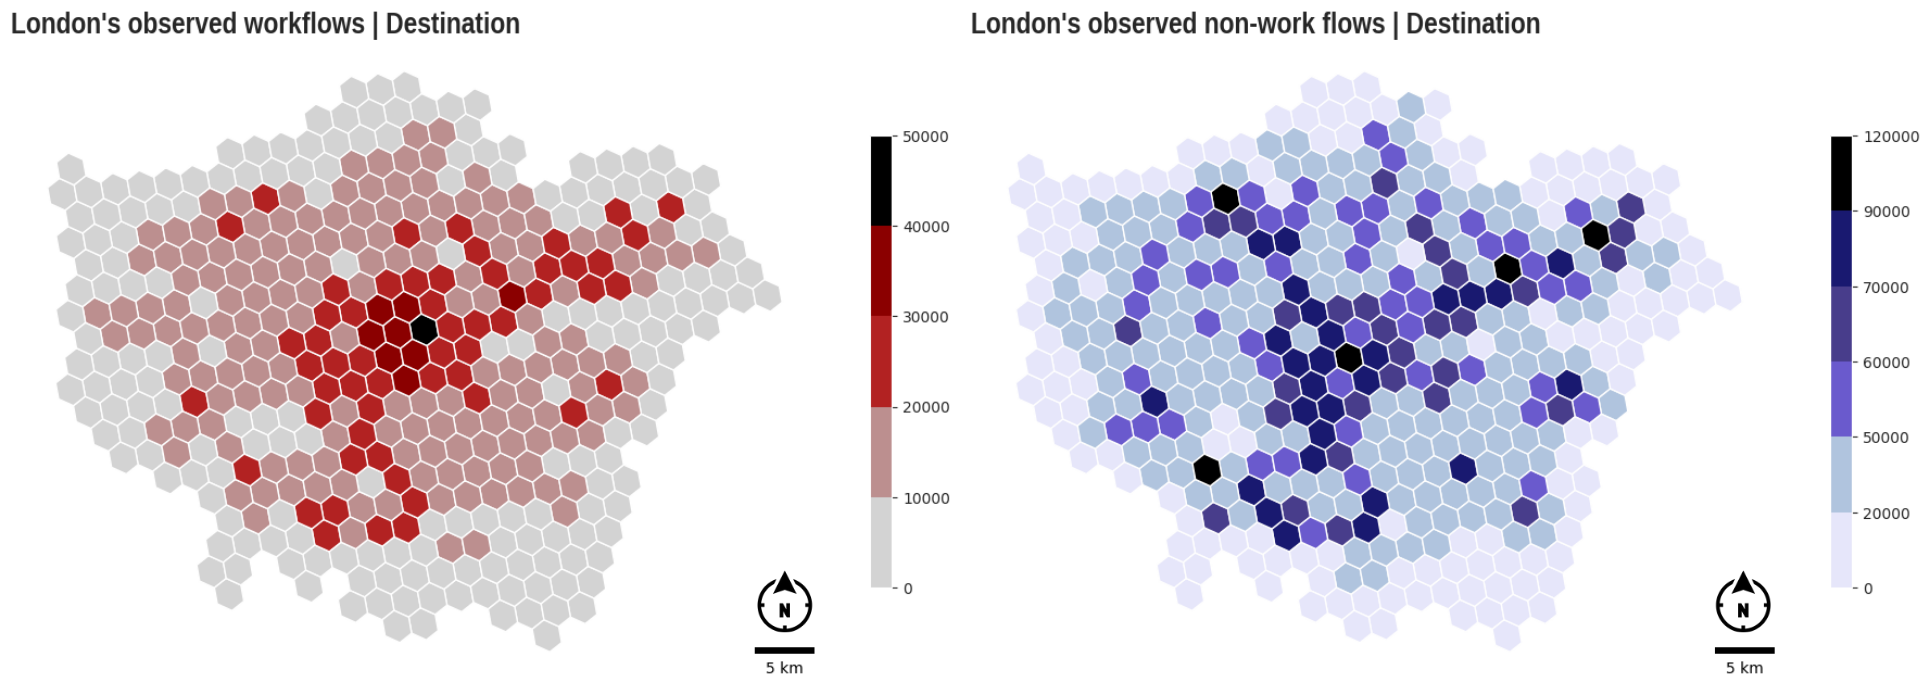
\includegraphics[width=15cm]{Images/Hex_observed_overview.png}
        \caption{London's observed flows: work and non-work.}
        \label{fig: observedflows_overview}
    \end{figure}

        \subsection{Features}


        

        \subsection{Attractiveness Factor}
        
        In the workflow regression analysis(Table \ref{tab:ols-results}), it is evident that the variables "EH," "PI," and "TR" have statistical significance since their p-values are low (all below 0.001). This indicates that these variables noticeably affect the dependent variable we are studying. Additionally, the high R-squared and adjusted R-squared values (0.863 and 0.860) signify that the model effectively explains much of the variation in the dependent variable.

        As part of the analytical refinement process, it was excluded the variables "CS" (commercial services) and "SE" (Sport and Entertainment). These variables were omitted due to their elevated p-values, above 0.4, signalling a lack of statistical significance. Additionally, both models exhibited a notably high condition number. However, a significant improvement was observed upon removing these two variables. The condition number, originally at 1.27e+03, was substantially reduced to a more manageable 647 in both regression models. 

\begin{table}[H]
\centering
\begin{tabular}{@{}lllll@{}}
\toprule
\textbf{Variables} & \textbf{coef} & \textbf{std err} & \textbf{P>|t|} \\ \midrule
Intercept & 932.6236 & 284.803 & 0.001 \\
AED & -14.0624 & 3.827 & 0.000 \\
AT & -42.8778 & 9.624 & 0.000 \\
\color[HTML]{9A0000} \textbf{EH} & \color[HTML]{9A0000} \textbf{33.2344} & \color[HTML]{9A0000} \textbf{6.902} & \color[HTML]{9A0000} \textbf{0.000} \\
MP & -32.6702 & 6.067 & 0.000 \\
\color[HTML]{9A0000} \textbf{PI} & \color[HTML]{9A0000} \textbf{80.2838} & \color[HTML]{9A0000} \textbf{6.608} & \color[HTML]{9A0000} \textbf{0.000} \\
RT & 5.8310 & 2.613 & 0.026 \\
\color[HTML]{9A0000} \textbf{TR} & \color[HTML]{9A0000} \textbf{18.1677} & \color[HTML]{9A0000} \textbf{6.916} & \color[HTML]{9A0000} \textbf{0.009} \\ \bottomrule
\textbf{R-squared} & 0.863 \\
\textbf{Adj. R-squared} & 0.860 \\
\textbf{Cond. No.} & 647. \\ \bottomrule
\hline
\end{tabular}
\caption{OLS Regression Results}
\label{tab:ols-results}
\end{table}

        Thus, within the context of workflows, the collective counts of Points of Interest from these three categories, namely "EH," "PI," and "TR," represent the Work-related Points of Interest. As shown in Figure \ref{fig: Regression_work}, these variables represent a linear relationship with the observed flows.

        \begin{figure}[H]
            \centering
            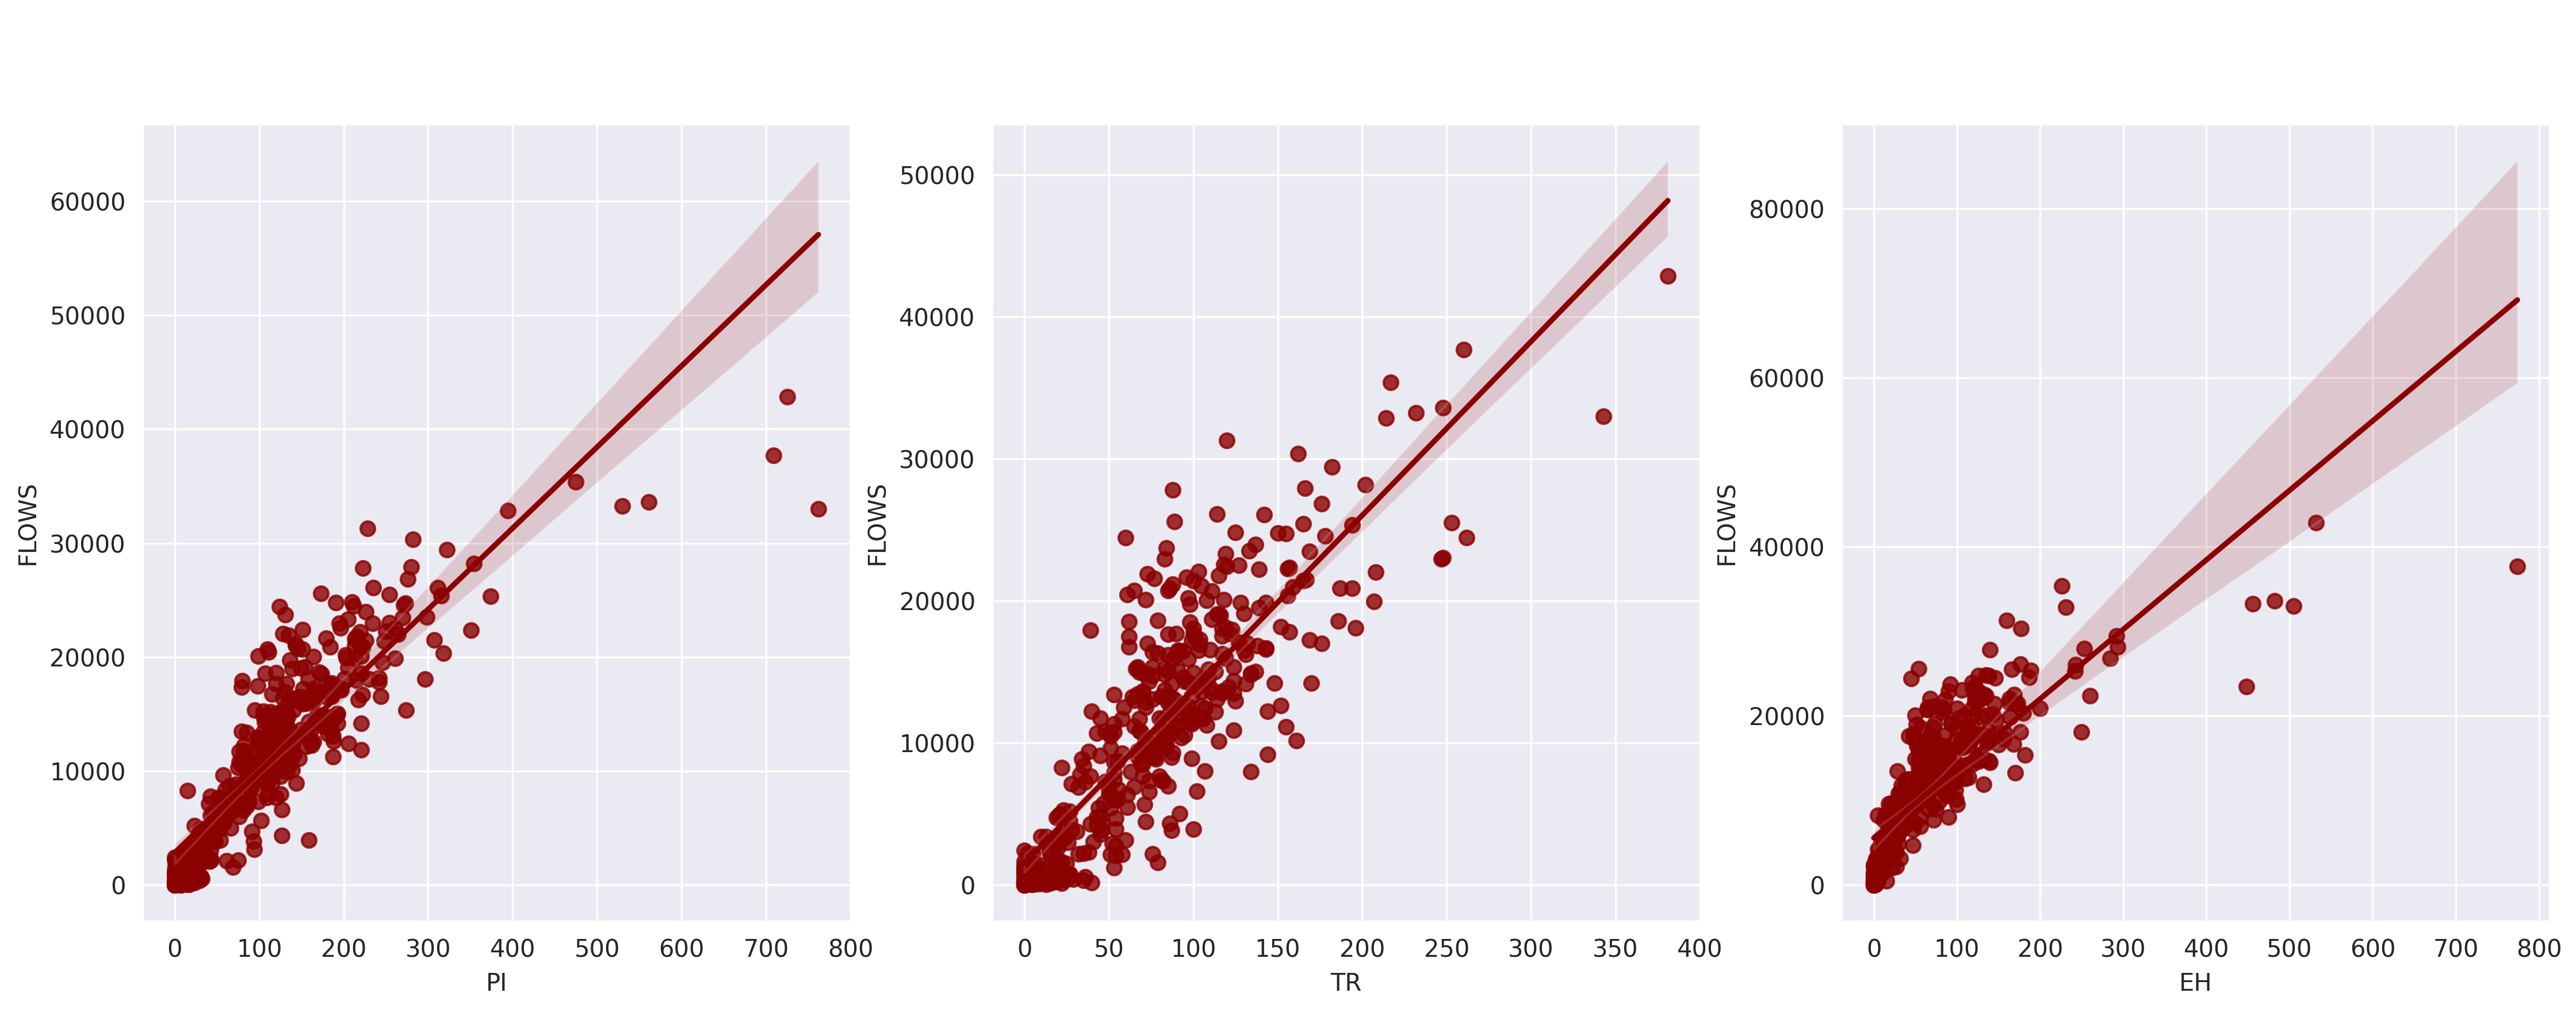
\includegraphics[width=14cm]{Images/regression_work.png}
            \caption{Work - Linear Regression: Flows vs POI}
            \label{fig: Regression_work}
        \end{figure}

        Regarding the non-work flows regression analysis in Table \ref{tab:ols-results-new-bold-color}, we observe that the variables "EH," "PI," "RT," and "TR" also demonstrate statistical significance, as their p-values are very low (all below 0.001). This implies that these variables significantly impact the dependent variable. The R-squared and adjusted R-squared values (0.782 and 0.778) indicate that our model effectively clarifies a significant portion of the variation in the dependent variable.  

        \begin{table}[H]
        \centering
        \begin{tabular}{@{}lllll@{}}
        \toprule
        \textbf{Variables} & \textbf{coef} & \textbf{std err} & \textbf{P>|t|} \\ \midrule
        Intercept & 5655.2406 & 1030.797 & 0.000 \\
        AED & -75.1430 & 13.851 & 0.000 \\
        AT & -201.4072 & 34.834 & 0.000 \\
        \textcolor{customblue}{\textbf{EH}} & \textcolor{customblue}{\textbf{113.3599}} & \textcolor{customblue}{\textbf{24.982}} & \textcolor{customblue}{\textbf{0.000}} \\
        MP & -131.6164 & 21.959 & 0.000 \\
        \textcolor{customblue}{\textbf{PI}} & \textcolor{customblue}{\textbf{218.6156}} & \textcolor{customblue}{\textbf{23.916}} & \textcolor{customblue}{\textbf{0.000}} \\
        \textcolor{customblue}{\textbf{RT}} & \textcolor{customblue}{\textbf{58.1842}} & \textcolor{customblue}{\textbf{9.456}} & \textcolor{customblue}{\textbf{0.000}} \\
        \textcolor{customblue}{\textbf{TR}} & \textcolor{customblue}{\textbf{73.5557}} & \textcolor{customblue}{\textbf{25.033}} & \textcolor{customblue}{\textbf{0.003}} \\ \bottomrule
        \textbf{R-squared} & 0.782 \\
        \textbf{Adj. R-squared} & 0.778 \\
        \textbf{Cond. No.} & 647. \\ \bottomrule
        \hline
        \end{tabular}
        \caption{OLS Regression Results}
        \label{tab:ols-results-new-bold-color}
        \end{table}

        In the non-work flows context, the combined counts of Points of Interest from these four categories, "EH," "PI," "RT," and "TR," symbolise the Non-Work-related Points of Interest. Thus, both regression models(Figure \ref{fig: Regression_nonwork}) appear well-suited for explaining the relationships between the independent and dependent variables.


        \begin{figure}[H]
            \centering
            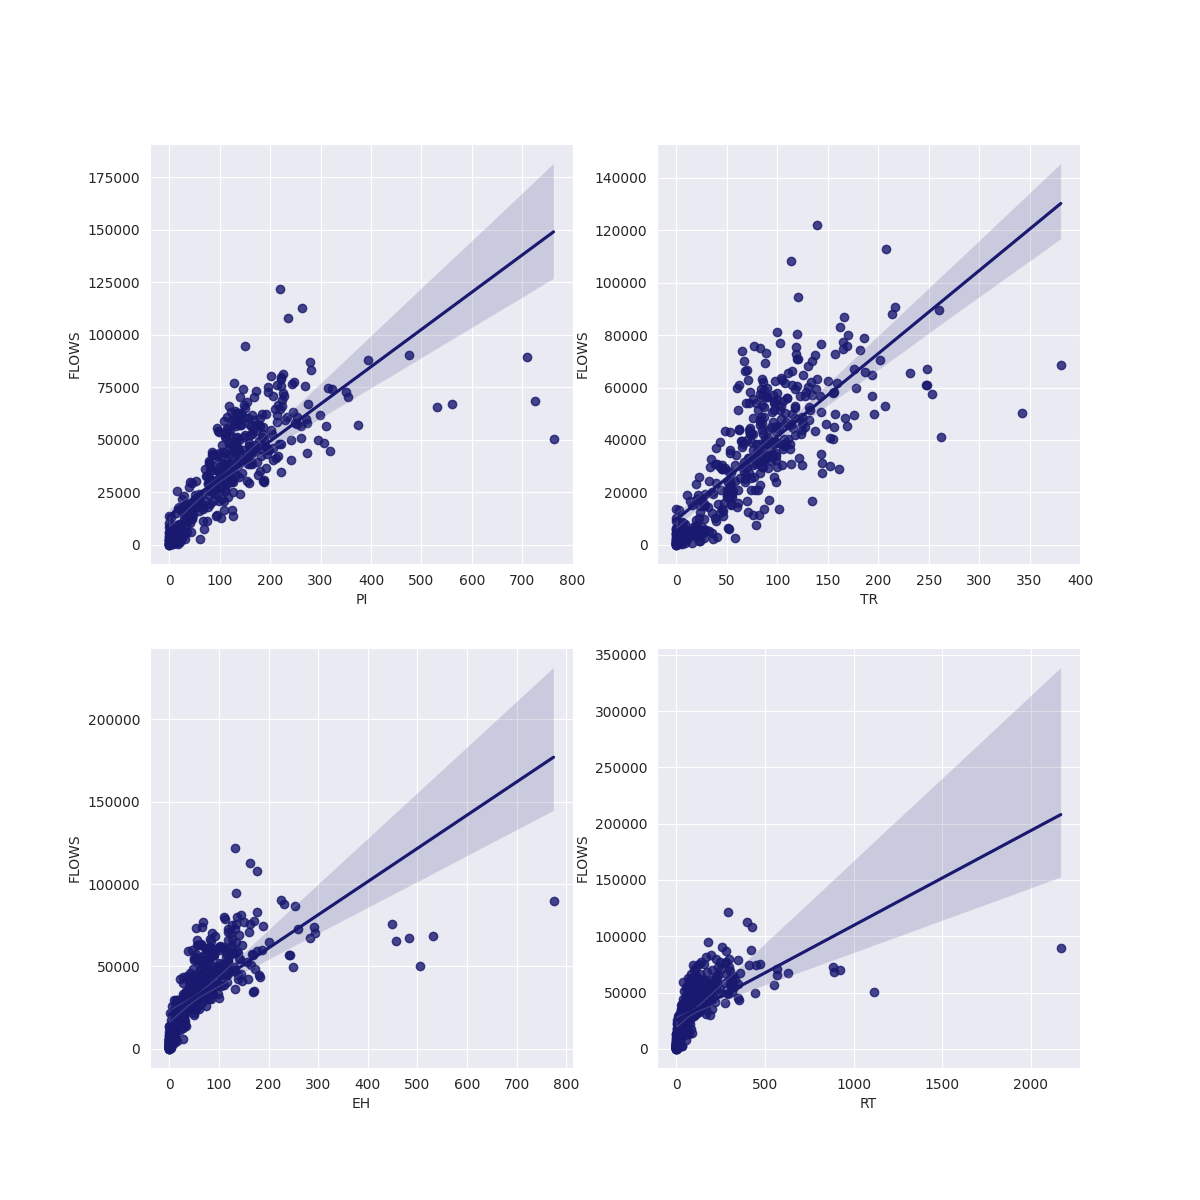
\includegraphics[width=14cm]{Images/regression_nonwork.png}
            \caption{Non-Work - Linear Regression: Flows vs POI}
            \label{fig: Regression_nonwork}
        \end{figure}


        In the context of residuals within both models(Figure \ref{fig: Residuals - Overview}), it is crucial to note that their distribution is normal, a fundamental assumption in regression analysis. This normal distribution holds significance because it indicates that errors in the model's predictions are distributed evenly around zero. Furthermore, the concentration of values is near zero when assessing the relationship between residuals and fitted values. This pattern confirms the suitability of the chosen linear regression models for the analysis.
        
        \begin{figure}[H]
            \centering
            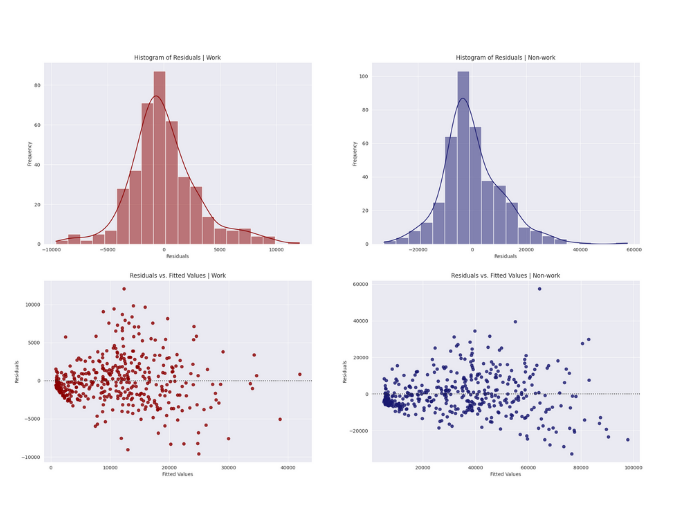
\includegraphics[width=14cm]{Images/Residuals_overview.png}
            \caption{Residuals - Overview}
            \label{fig: Residuals - Overview}
        \end{figure}
        
 

        The map below(Figure \ref{fig: POI_map}) illustrates the spatial distribution of Points of Interest (POI) in London, categorising them into work-related and non-work-related. It becomes evident that their distribution across the city exhibits a degree of similarity, predominantly concentrating in inner London instead of outer London. However, it is worth emphasising that the total number of points differs significantly due to the non-work category that contains four distinct POI groups. The POI values for non-work are also correlated with mobility flow values distribution, as the proportions remain consistent. Work-related flows represent only a fraction of the city's overall journeys, whereas non-work flows encompass a broader spectrum of activities.

        \begin{figure}[H]
            \centering
            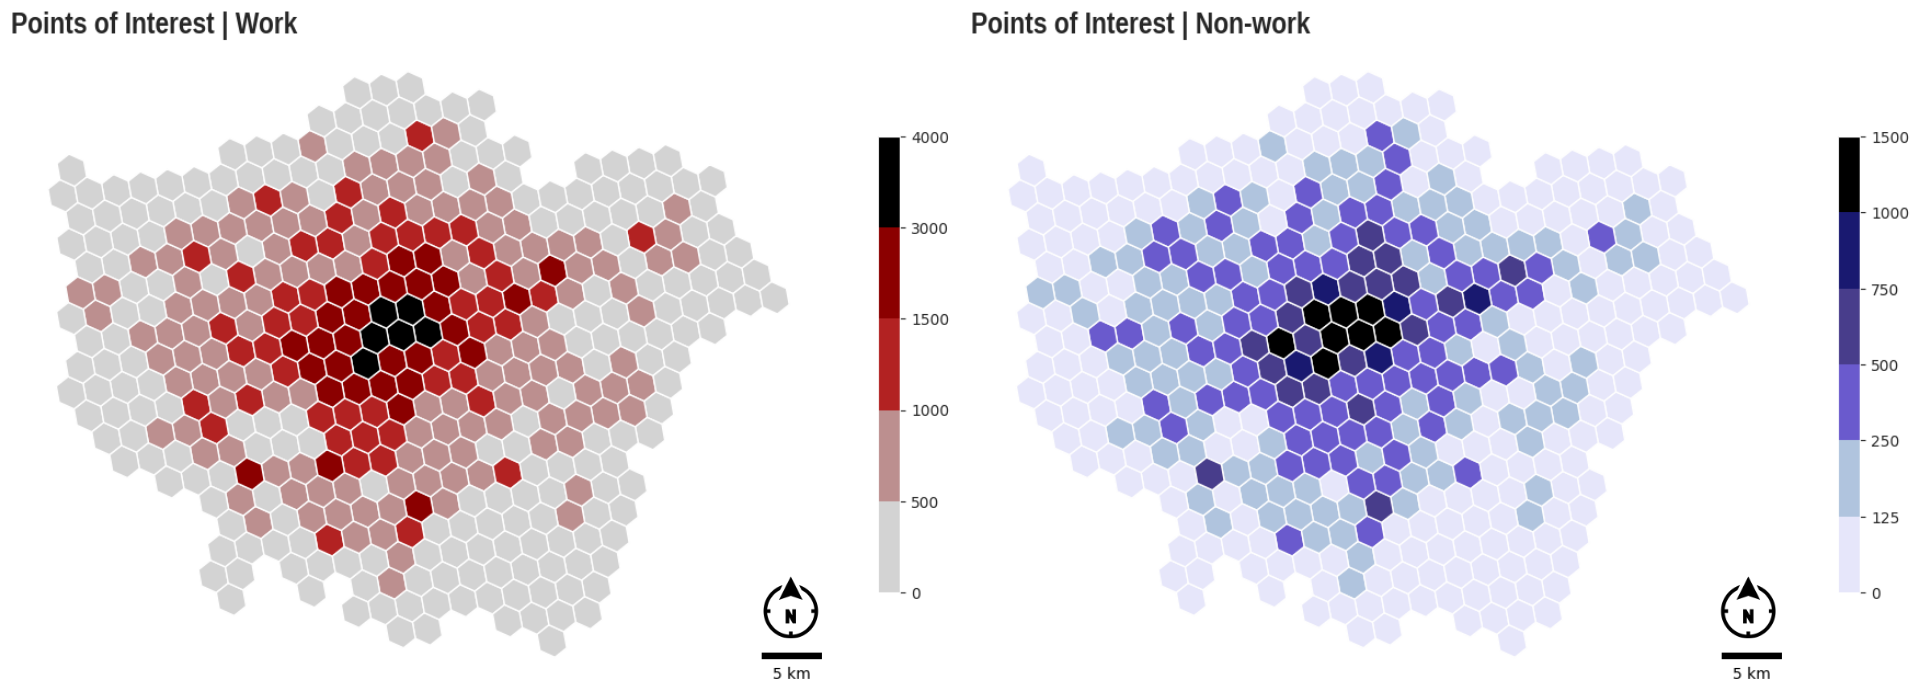
\includegraphics[width=14cm]{Images/POI_map.png}
            \caption{Points of Interest spatial distribution: Work and Non-work}
            \label{fig: POI_map}
        \end{figure}

        Additionally, the analysis reveals varying concentration patterns between the two categories of amenities. Work-related amenities exhibit a higher concentration in the city centre, whereas non-work amenities exhibit a more gradual and dispersed distribution throughout the city. This nuanced spatial distinction highlights these amenities' differential nature and accessibility for London's residents and visitors.

        \subsection{Population}
 
        To standardise the data, the 2021 census population data was aggregated, aligning it with the level 7 hexagons, as visually represented in the map below(Figure \ref{fig: Population Census}). This aggregation illustrate a significant concentration of residents within inner London, especially within the northeastern quadrant. While some other areas display a more dispersed spatial distribution, central London's concentration closely reflects the distribution patterns evident in the Points of Interest dataset and the mobility flows data.
        
        \begin{figure}[H]
            \centering
            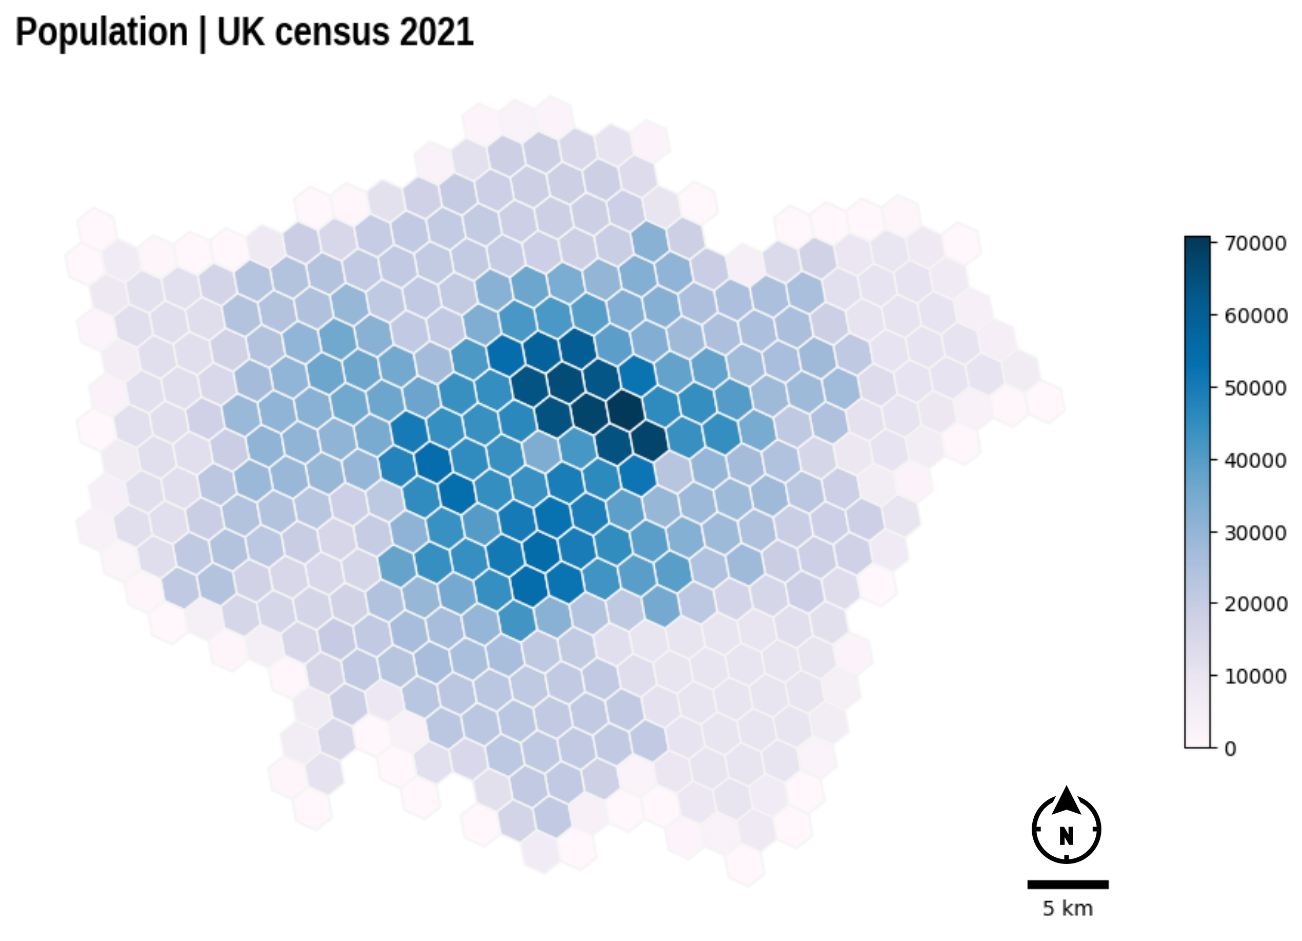
\includegraphics[width=12cm]{Images/population.png}
            \caption{Population - UK Census 2021}
            \label{fig: Population Census}
        \end{figure}
    
    \section{Analyzing the models comparatively}  

    The application of the spatial interaction model revealed limitations when processing the large dataset from the Mobility dataset. However, in contrast, the Deep Gravity Model demonstrated exceptional predictive capabilities, even in the face of substantial data volumes. The deep gravity model showcased its effectiveness when analyzing hexagons up to level 9, encompassing a vast geographical expanse of 17,636 hexagons and offering over 300 million potential origin-destination flows. On the other hand, the spatial interaction model was limited. It was restricted to operating exclusively within hexagons at level 7, where it relied upon the computational of a GPU equipped with high-performance RAM.

    The architecture of the Deep Gravity Model entails a division of geographic region units into distinct training and test groups, a feature that has contributed to its challenges in effectively managing Big Datasets. Consequently, the model generates results exclusively for the training sample. Therefore, to maintain the integrity and consistency in our comparative analysis across various models and flow types, we opted to employ the same sample for the Production-Constrained Model, aligning it with the dataset utilised for the Deep Gravity Model. This approach ensured a comprehensive and meaningful evaluation of model performance and the complex flow dynamics patterns aimed to uncover and understand.

    Some key findings in the regression plot(\ref{fig: Flows - Regression}) illustrate the relationship between the observed flows and those generated by the Deep Gravity Model (DG) and the Spatial Interaction Model (SIM). Therefore, the plot reveals a linear relationship on relationship between these variables. Furthermore, the graph unveils distinctive characteristics in the distribution of data values for each flow type. Specifically, when we examine the non-work flows, they exhibit a higher concentration, with values clustering closer to zero on the graph. In contrast, the non-work flows display a more dispersed pattern, with values distributed across a wider range of values. This divergence in the distribution patterns of the two flow types is a significant finding drawn from the regression plot. It emphasises the need for a differentiated analytical approach for each flow type.

            \begin{figure}[H]
            \centering
            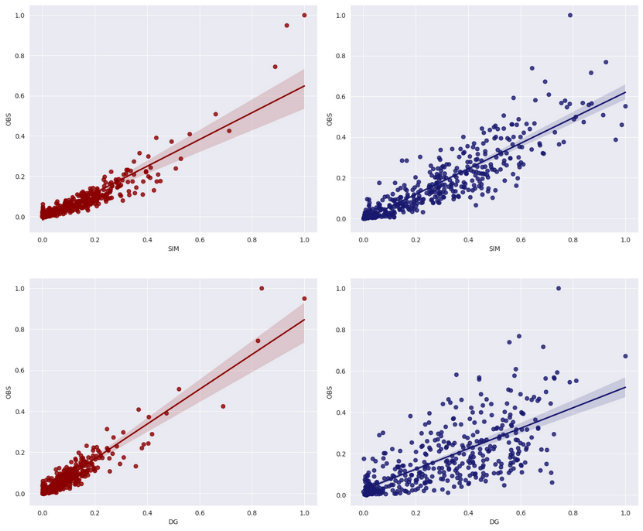
\includegraphics[width=14cm]{Images/Flows_regression.png}
            \caption{Flows - Regression plot}
            \label{fig: Flows - Regression}
            \footnotesize{\textbf{Red:} Workflows. \textbf{Blue:} Non-work flows.}
        \end{figure}

    In assessing the performance of the models in predicting flows, it is evident that the R-squared values for Non-work flows outperform those for workflows, with a notable high value of 0.7 observed in the production-constrained model for non-work flows and 0.9 in the Deep Gravity Model. In the context of workflows, the DG model achieved a better performance of 0.9, while the SIM model had 0.6.
    
    R-squared serves as a valuable metric for comprehending the influence of variables on flow prediction. Consequently, it becomes crucial to measure the efficacy of each model in estimating flows and the capability of selected independent variables in predicting the outcome. Among these variables, including distance, population, and the attractiveness factor derived from Points of Interest (POI), it is evident that they demonstrate superior performance in estimating flows, particularly within the Deep gravity model, outperforming the SIM model. Because of that, evaluating the Root Mean Square Error (RMSE) arises as an essential measure for comparing and evaluating the models against each other.

    The performance of the models displayed significant variations depending on the specific type of flow under consideration. It is important to highlight that the Production-Constrained Model, when put to the test, yielded the lowest RMSE value, achieving a relevant score of 14.69 for work-related flows. On the other hand, the Deep Gravity Model showcased a significantly lower RMSE value as well, standing at 41.47 for workflows. The model performance across these different flow types is concisely summarised in Table \ref{table: RMSE}, providing a comprehensive overview of how each model excelled in distinct aspects of mobility prediction.

            \begin{table}[h]
        \centering
        \begin{tabular}{@{}lll@{}}
        \toprule
        \textbf{Flows type} & \textbf{Deep Gravity} & \textbf{Production-Constrained} \\ \midrule
        Work                & 41.47                & 14.69                          \\
        Non-work            & 336.71                 & 141.19                          \\ \bottomrule
        \end{tabular}
            \caption{RMSE}
            \label{table: RMSE}
        \end{table}
    
    The contrast in model performance reveals a pattern: Models rooted in deep learning structures outperform the production-constrained model when predicting workflows. This result is evidenced by the high r-squared values and low RMSE (Root Mean Square Error) associated with these models. On the other hand, the prediction of non-work flows reveals a more complex context characterised by non-linear trajectories within the urban environment. Thus, both models achieve high r-squared values, with the deep gravity model slightly edging ahead. However, the SIM model records a lower RMSE value than the deep gravity model in this context.

    Nevertheless,  despite the spatial interaction model's computational limitations, the deep gravity model performs better when handling larger datasets. This is exemplified in Table \ref{table: RMSE_DG}, where the model demonstrates an r-squared of 0.7, lower than what was achieved at level 7. However, it is worth noting that the deep gravity model yields a lower RMSE, specifically 28.01, higher than the corresponding figure for the SIM model. Therefore, when the model aggregates data, the DG model experiences a decrease in performance in terms of RMSE, indicating the specificities of model behaviour under varying data conditions.
        
        \begin{table}[H]
        \centering
        \begin{tabular}{@{}lll@{}}
        \toprule
        \textbf{Flows type} & \textbf{Level 8} & \textbf{Level 7} \\ \midrule
        Work                & 433.65                & 41.47                          \\
        Non-work            & 28.01                 & 336.71                          \\ \bottomrule
        \end{tabular}
            \caption{RMSE- Deep Gravity Model at Hexagons level 7 and 8}
            \label{table: RMSE_DG}
        \end{table}
    
    
    In this context, the non-work flows contain various activities and behaviours within a city, such as leisure, tourism, and social interactions. These activities tend to follow less predictable patterns, making them challenging to model accurately. However, with its inherent capacity to capture intricate relationships and dependencies within the data, the Deep Gravity Model excelled in this aspect. It showcased its ability to predict the diverse and sometimes complex mobility patterns associated with non-work-related activities, producing lower error rates.
    
    The traditional Spatial Interaction Model demonstrated its comparative advantage in estimating flows characterised by a more linear and structured relationship, primarily those about work-related activities. Workflows often follow established commuting routes and daily routines, resulting in more predictable mobility patterns. In these scenarios, the traditional model indicated greater accuracy in the workflow predictions. However, it obtained an RMSE rate for non-workflows.
        
    To compared the models, values were normalised.
        
        \begin{figure}[H]
            \centering
            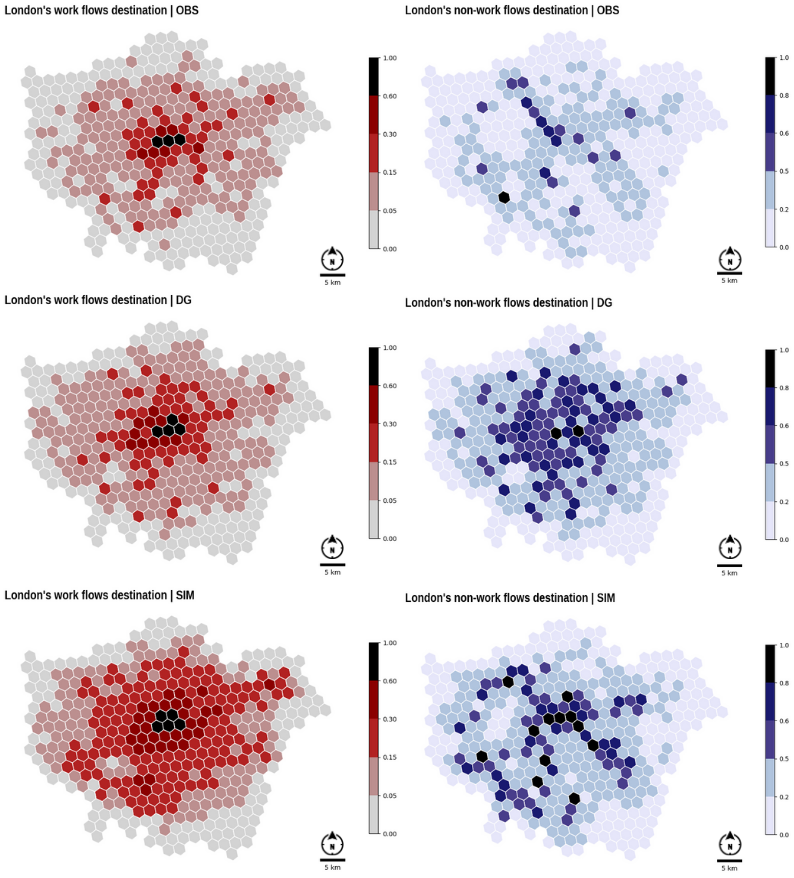
\includegraphics[width=15cm]{Images/Hex_comparativeanalysis.png}
            \caption{Observed and predicted flows for work and non-work flows}
            \footnotesize{OBS: Observed, DG: Deep Gravity, SIM: Spatial Interaction model, Red: workflows, Blue: non-workflows}
            \label{fig: nWF Model after calibration}
        \end{figure}

%%%%%%%%%%%%% DISCUSSION
        
\section{Discussion}

       The attractiveness factor utilised in the Spatial Interaction Model for Work and Non-work flows was constructed based on the categories within the POI dataset; see Figure \ref{fig: Attractiveness factor}. In the context of Workflows, the analysis revealed that Public Infrastructure (PI), Transport (TR), and Education and Health (EH) emerged as the most significant variables in the data collected from Mobility Data. In contrast, for the Non-work attractiveness factor, the primary variables align with those of the Workflows, except for Retail (RT).

        \begin{figure}[H]
            \centering
            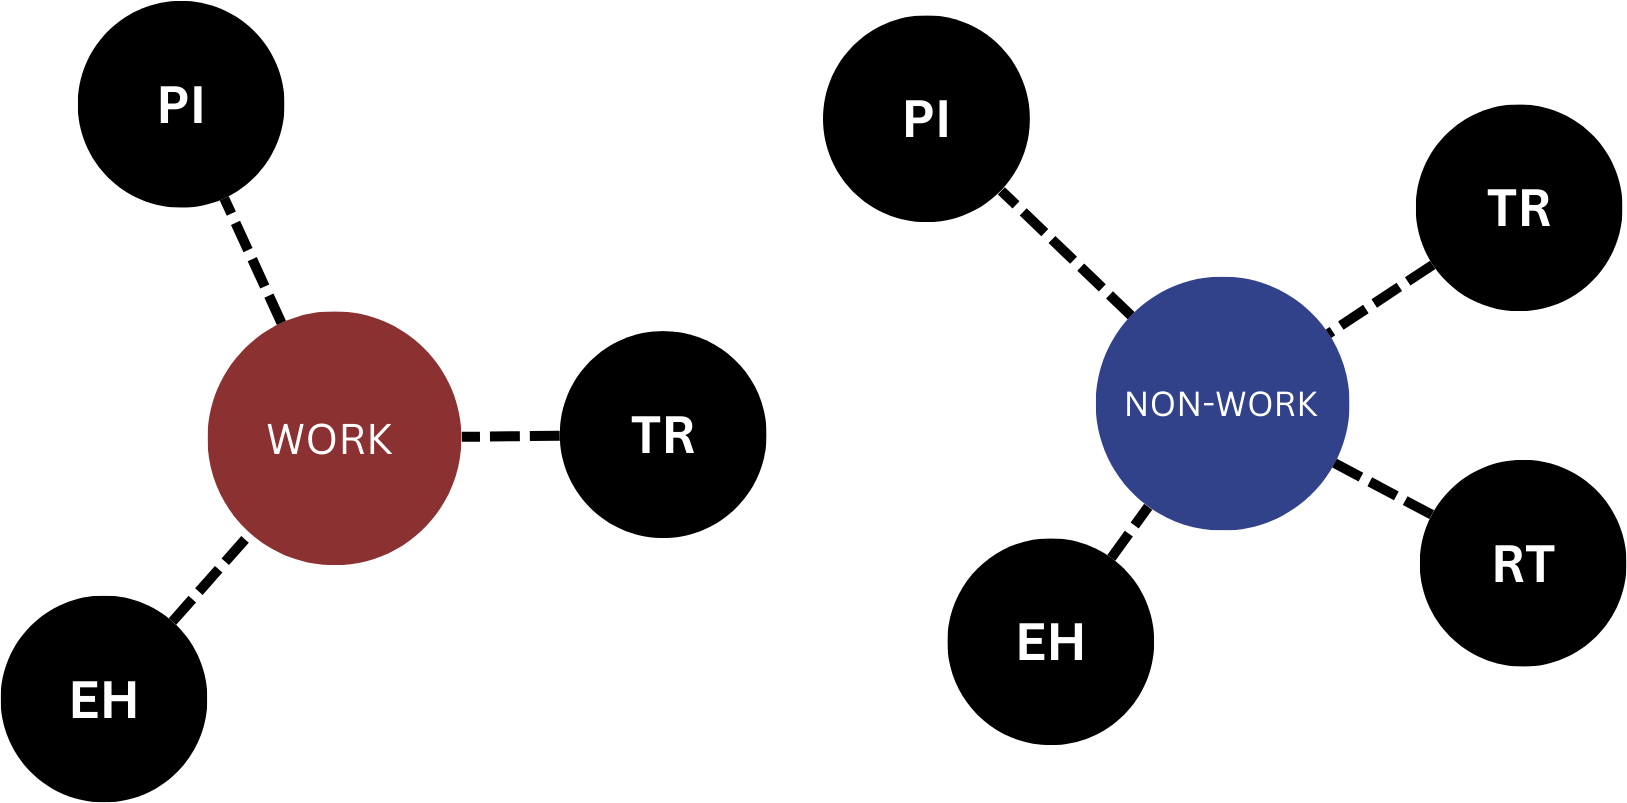
\includegraphics[width=14cm]{Images/Atractiveness factor.png}
            \caption{Attractiveness factor}
            \label{fig: Attractiveness factor}
        \end{figure}

        This outcome provides valuable insights into the correlation of these two types of flows concerning user destinations. However, it is essential to note that the presence of these Points of Interest does not imply that they exclusively represent places of work or leisure destinations. It signifies the concentration of these amenity categories within specific geographic regions(hexagons), where opportunities for work or leisure coexist.

        To illustrate this, in the context of workflows, the coexistence of Points of Interest related to Public Infrastructure, Transport, Education, and Health suggests a likely concentration of work-related activities within that region. On the other hand, Non-work flows, including Retail as a relevant variable, are intriguing, as they pertain to flows unrelated to work, encompassing activities like visiting parks, schools, and cafes. Consequently, the aggregation of these four types of amenities is closely linked to the destinations of individuals in London who are not primarily there for work-related purposes.
        
        In the course of this study, a series of critical questions deserve careful consideration:
        
        Firstly, evaluating the relative performance of the Deep Gravity Model in estimating carbon emissions within the London area is essential. This assessment provides valuable insights into the model's effectiveness in capturing the complex dynamics of carbon emissions, which is crucial for understanding urban environmental impact.
        
        Secondly, the combined analysis of the Deep Gravity Model with accessibility measures presents a crucial path for investigation. This integration can enhance the model's predictive capacity by leveraging accessibility data, providing a more comprehensive understanding of the factors influencing carbon emissions.
        
        However, it is crucial to consider the limitations inherent in this analysis. Specifically, a need exists to enrich the features set, with a notable example being the incorporation of detailed street network information, as applied in the original model. Additionally, accounting for significant external variables such as weather conditions or events like strikes, which can significantly impact the mobility flows dynamic, is crucial to address the model's complexities.
        
        Besides that, it is crucial to consider additional performance metrics that can comprehensively assess the Deep Gravity Model's effectiveness relative to alternative methodologies to ensure a robust comparison.This broader perspective facilitates a comprehensive understanding of the strengths and weaknesses of each model, leading to more informed conclusions regarding their respective capabilities in mobility flow estimation. 

        Utilizing the mobility dataset from Locomizer has proven valuable for analyzing commuting dynamics. The data employed in this study is as recent as March, while the Census data concerning origin and destination data from 2011. Although these databases primarily have the retail market as one of their main audiences, their relevance extends far beyond, including urban planning. They offer a unique lens through which to comprehend the ever-evolving dynamics of cities, influenced by factors as diverse as climate crises, marked by intense weather fluctuations, and socioeconomic variables like recent strikes affecting various sectors in England.

        Locomizer's dataset has a range of possibilities for spatial analysis, and many still need to be explored within the scope of this study. It holds the potential to solve travel patterns based on transportation modes and varying times of day to understand how these factors impact the city's fabric throughout the day.
        
        Regarding features, this analysis has focused primarily on geographical data linked to the points of interest dataset. However, the Deep Gravity Model, which can accommodate up to 18 features in its vector, offers opportunities for greater complexity. Integrating additional databases like OpenStreetMap could add a deeper understanding of the study area's geographical intricacies, reflecting mobility patterns and the factors driving people's movements within the city.
        
        Including the population census dataset proved instrumental in running the four models. Nevertheless, it would be of immense value if Locomizer's Mobility data could provide information on the "Visitation Modality" beyond just worker users and residents. While the dataset's documentation indicates the availability of this information, the version used in this research did not include it. Access to resident data would enhance data integrity and offer insights into user movement patterns within the same Locomizer data ecosystem.
        
        The remarkable performance of the Deep Gravity Model stands out, even when handling substantial datasets. The model's capability extends to analysing hexagons up to level 9, encompassing 17,636 hexagons and 300 million origin and destination possibilities. Therefore, it underscores the potential of employing cutting-edge models and incorporating machine learning techniques like deep learning to tackle the complexity of contemporary databases that demand enhanced computational capabilities.
        
        The primary concern is that the two primary metrics commonly utilised in this context, namely R2 and RMSE/SRMSE, have previously been indicated as inadequate representations of the actual inherent model performance due to the unique characteristics of spatial interaction flow. Consequently, this can result in erroneous deductions regarding relative performance (Knudsen \& Fotheringham, 1986) \cite{wilkinsonSpatialInteractionModels2023}
        
        Lastly, the scope of this analysis is limited to a specific day of the year. A broader temporal evaluation, encompassing an extended period, would greatly contribute to understanding the model's performance over time, enabling insights into its stability and consistency across varying time frames.

        Despite the complexity of the datasets involved, particularly the Mobility Data, and the inclusion of multiple models (totalling four models), the principal focus of this study remains centred on utilising RMSE as the primary parameter and supplementing it with R-squared for individual model performance.

        However, it is crucial to acknowledge the limitations \cite{wilkinsonSpatialInteractionModels2023} outlined for a more comprehensive analysis. As emphasized by Wilkinson, when assessing the efficacy of spatial interaction models, it becomes crucial to account for the outcomes generated by these models, ensuring their alignment with the dataset. He warns against only using a single metric for evaluation, as such an approach might generate inaccurate conclusions regarding modelling performance. Thus, it resonates with the view that an evaluation is necessary to avoid misguided interpretations.
        
        Furthermore, \cite{wilkinsonSpatialInteractionModels2023} highlights a key consideration - the overall usage of two key metrics, R-squared and RMSE/SRMSE, may not necessarily capture the genuine underlying performance of a model. It is attributed to the inherent characteristics of spatial interaction flow, leading to potential inaccuracies in determining relative performance. Knudsen and Fotheringham (1986) suggest that these metrics might only partially reflect the true model performance due to the complex dynamics inherent in spatial interaction.
        
        Combining these perspectives, it is evident that while RMSE and R-squared offer valuable insights, their limitations must be acknowledged. Particularly, the exclusion of additional evaluation criteria and the potential inadequacy of certain metrics in capturing complex spatial dynamics need to be recognised. Additionally, as Wilkinson (2023) recommends, understanding how different features and datasets contribute to model performance is vital, especially in scenarios involving the integration of new datasets
        







\chapter{Conclusions}
\label{chapterlabel4}

% This just dumps some pseudolatin in so you can see some text in place.
%\blindtext



\addcontentsline{toc}{chapter}{Appendices}

% The \appendix command resets the chapter counter, and changes the chapter numbering scheme to capital letters.
%\chapter{Appendices}
\appendix
\chapter{Features Classification}
\label{appendices1}

\begin{table}[H]
\begin{tabular}{lll}
\hline
{\color[HTML]{000000} \textbf{Feature}}                            & {\color[HTML]{000000} \textbf{Group}} & {\color[HTML]{000000} \textbf{Categories/Group}}                                                                                                                                                                                                                                           \\ \hline
Bus stops                                                          & TR                                    & Bus Transport                                                                                                                                                                                                                                                                              \\ \hline
Public Transport                                                   & TR                                    & Public Transport, Stations and Infrastructure                                                                                                                                                                                                                                              \\ \hline
Water                                                              & TR                                    & Water                                                                                                                                                                                                                                                                                      \\ \hline
Air                                                                & TR                                    & Air                                                                                                                                                                                                                                                                                        \\ \hline
Education                                                          & EH                                    & \begin{tabular}[c]{@{}l@{}}Recreational and Vocational Education; \\ Primary, Secondary and Tertiary Education;\\ Education Support Services\end{tabular}                                                                                                                                  \\ \hline
Health                                                             & EH                                    & \begin{tabular}[c]{@{}l@{}}Health Support Services; Animal Welfare;\\ Health Practitioners and Establishments\end{tabular}                                                                                                                                                                 \\ \hline
Accomodation                                                       & AED                                   & \begin{tabular}[c]{@{}l@{}}Banqueting and Function Rooms; Camping, \\ Caravanning, Mobile Homes, Holiday \\ Parks and Centres; Timeshare; Bed and \\ Breakfast and Backpacker Accommodation; \\ Self Catering Youth Accommodation; \\ Hotels, Motels, Country Housesand Inns;\end{tabular} \\ \hline
Restaurants                                                        & AED                                   & Restaurants                                                                                                                                                                                                                                                                                \\ \hline
Fast Food                                                          & AED                                   & \begin{tabular}[c]{@{}l@{}}Fast Food and Takeaway Outlets; Fish and \\ Chip Shops; Fast Food Delivery Services\end{tabular}                                                                                                                                                                \\ \hline
Pubs, Bars and Inns                                                & AED                                   & Pubs, Bars and Inns                                                                                                                                                                                                                                                                        \\ \hline
Cafes                                                              & AED                                   & Cafes, Snack Bars and Tea Rooms; Internet Cafes                                                                                                                                                                                                                                            \\ \hline
Retail                                                             & RT                                    & Group                                                                                                                                                                                                                                                                                      \\ \hline
Commercial services                                                & CS                                    & Group                                                                                                                                                                                                                                                                                      \\ \hline
\begin{tabular}[c]{@{}l@{}}Sport and \\ Entertainment\end{tabular} & SE                                    & Group                                                                                                                                                                                                                                                                                      \\ \hline
Attractions                                                        & AT                                    & Group                                                                                                                                                                                                                                                                                      \\ \hline
Infrastructure                                                     & PI                                    & Infrastructure and Facilities                                                                                                                                                                                                                                                              \\ \hline
Government                                                         & PI                                    & Central and Local Government                                                                                                                                                                                                                                                               \\ \hline
Organisations                                                      & PI                                    & Organisations                                                                                                                                                                                                                                                                              \\ \hline
\end{tabular}
\caption{Table Caption}
\end{table}

%%%%%%%%%%%%%%%%%%%%%%%%%%%%%%%%%%
\chapter{Code availability}
\label{appendices2}

    The Python code and the Latex code of this dissertation are available at \href{https://github.com/brfelipealmeida/LondonMobilityFlows}{https://github.com/brfelipealmeida/LondonMobilityFlows}
    
%%%%%%%%%%%%%%%%%%%%%%%%%%%%%%%%%%
\chapter{Meetings with supervisors}
\label{appendices3}

\begin{table}[h]
\centering
\begin{tabular}{lllll}
\hline
\textbf{Nº} & \textbf{Date} & \textbf{Topic} & \textbf{Supervisor} & \textbf{Type} \\
\hline
01 & 12/04/2023 & Introduction & Elsa & Online \\
02 & 14/04/2023 & Introduction with Project Partner & Elsa, Mateo & Online \\
03 & 16/05/2023 & Literature Review and Methodology & Elsa & CASA \\
04 & 09/06/2023 & Group Presentation & Elsa, Mateo & CASA \\
05 & 13/06/2023 & Methodologies and Datasets & Mateo Neira & Online \\
06 & 23/06/2023 & Methodology & Elsa & Online \\
07 & 06/07/2023 & Locomizer dataset Meeting & Mateo Neira & Online \\
08 & 11/07/2023 & Skeleton & Elsa & CASA \\
09 & 18/07/2023 & Locomizer dataset & Elsa, Mateo & Online \\
10 & 20/07/2023 & Results & Elsa & CASA \\
11 & 28/07/2023 & Results & Elsa & CASA \\
\hline
\end{tabular}
\caption{Table Caption}
\end{table}




%\addcontentsline{toc}{chapter}{Appendices}

% The \appendix command resets the chapter counter, and changes the chapter numbering scheme to capital letters.
%\chapter{Appendices}
\appendix
\chapter{Features Classification}
\label{appendices1}

\begin{table}[H]
\begin{tabular}{lll}
\hline
{\color[HTML]{000000} \textbf{Feature}}                            & {\color[HTML]{000000} \textbf{Group}} & {\color[HTML]{000000} \textbf{Categories/Group}}                                                                                                                                                                                                                                           \\ \hline
Bus stops                                                          & TR                                    & Bus Transport                                                                                                                                                                                                                                                                              \\ \hline
Public Transport                                                   & TR                                    & Public Transport, Stations and Infrastructure                                                                                                                                                                                                                                              \\ \hline
Water                                                              & TR                                    & Water                                                                                                                                                                                                                                                                                      \\ \hline
Air                                                                & TR                                    & Air                                                                                                                                                                                                                                                                                        \\ \hline
Education                                                          & EH                                    & \begin{tabular}[c]{@{}l@{}}Recreational and Vocational Education; \\ Primary, Secondary and Tertiary Education;\\ Education Support Services\end{tabular}                                                                                                                                  \\ \hline
Health                                                             & EH                                    & \begin{tabular}[c]{@{}l@{}}Health Support Services; Animal Welfare;\\ Health Practitioners and Establishments\end{tabular}                                                                                                                                                                 \\ \hline
Accomodation                                                       & AED                                   & \begin{tabular}[c]{@{}l@{}}Banqueting and Function Rooms; Camping, \\ Caravanning, Mobile Homes, Holiday \\ Parks and Centres; Timeshare; Bed and \\ Breakfast and Backpacker Accommodation; \\ Self Catering Youth Accommodation; \\ Hotels, Motels, Country Housesand Inns;\end{tabular} \\ \hline
Restaurants                                                        & AED                                   & Restaurants                                                                                                                                                                                                                                                                                \\ \hline
Fast Food                                                          & AED                                   & \begin{tabular}[c]{@{}l@{}}Fast Food and Takeaway Outlets; Fish and \\ Chip Shops; Fast Food Delivery Services\end{tabular}                                                                                                                                                                \\ \hline
Pubs, Bars and Inns                                                & AED                                   & Pubs, Bars and Inns                                                                                                                                                                                                                                                                        \\ \hline
Cafes                                                              & AED                                   & Cafes, Snack Bars and Tea Rooms; Internet Cafes                                                                                                                                                                                                                                            \\ \hline
Retail                                                             & RT                                    & Group                                                                                                                                                                                                                                                                                      \\ \hline
Commercial services                                                & CS                                    & Group                                                                                                                                                                                                                                                                                      \\ \hline
\begin{tabular}[c]{@{}l@{}}Sport and \\ Entertainment\end{tabular} & SE                                    & Group                                                                                                                                                                                                                                                                                      \\ \hline
Attractions                                                        & AT                                    & Group                                                                                                                                                                                                                                                                                      \\ \hline
Infrastructure                                                     & PI                                    & Infrastructure and Facilities                                                                                                                                                                                                                                                              \\ \hline
Government                                                         & PI                                    & Central and Local Government                                                                                                                                                                                                                                                               \\ \hline
Organisations                                                      & PI                                    & Organisations                                                                                                                                                                                                                                                                              \\ \hline
\end{tabular}
\caption{Table Caption}
\end{table}

%%%%%%%%%%%%%%%%%%%%%%%%%%%%%%%%%%
\chapter{Code availability}
\label{appendices2}

    The Python code and the Latex code of this dissertation are available at \href{https://github.com/brfelipealmeida/LondonMobilityFlows}{https://github.com/brfelipealmeida/LondonMobilityFlows}
    
%%%%%%%%%%%%%%%%%%%%%%%%%%%%%%%%%%
\chapter{Meetings with supervisors}
\label{appendices3}

\begin{table}[h]
\centering
\begin{tabular}{lllll}
\hline
\textbf{Nº} & \textbf{Date} & \textbf{Topic} & \textbf{Supervisor} & \textbf{Type} \\
\hline
01 & 12/04/2023 & Introduction & Elsa & Online \\
02 & 14/04/2023 & Introduction with Project Partner & Elsa, Mateo & Online \\
03 & 16/05/2023 & Literature Review and Methodology & Elsa & CASA \\
04 & 09/06/2023 & Group Presentation & Elsa, Mateo & CASA \\
05 & 13/06/2023 & Methodologies and Datasets & Mateo Neira & Online \\
06 & 23/06/2023 & Methodology & Elsa & Online \\
07 & 06/07/2023 & Locomizer dataset Meeting & Mateo Neira & Online \\
08 & 11/07/2023 & Skeleton & Elsa & CASA \\
09 & 18/07/2023 & Locomizer dataset & Elsa, Mateo & Online \\
10 & 20/07/2023 & Results & Elsa & CASA \\
11 & 28/07/2023 & Results & Elsa & CASA \\
\hline
\end{tabular}
\caption{Table Caption}
\end{table}



 
% You could separate these out into different files if you have
%  particularly large appendices.

% This line manually adds the Bibliography to the table of contents.
% The fact that \include is the last thing before this ensures that it
% is on a clear page, and adding it like this means that it doesn't
% get a chapter or appendix number.


%\renewcommand{\bibname}{References}
% Actually generates your bibliography.

\renewcommand{\bibname}{References}
\bibliographystyle{agsm}
\bibliography{References.bib}
\addcontentsline{toc}{chapter}{Bibliography}


% All done. \o/
\end{document}
